\documentclass[notoc]{JHEP3}
\usepackage{cite,color,psfrag,url,latexsym,graphicx,epstopdf,slashed,xspace,hyperref,enumitem,lineno}
\let\normalcolor\relax

\newcommand{\nn}{\nonumber \\}
\newcommand{\pt}{$p_{T}$}
\newcommand{\eqref}[1]{(\ref{#1})}
\newcommand{\text}[1]{{\rm #1}}
\newcommand{\jw}{\textsc{Jewel}~}
\newcommand{\jwpy}{\textsc{Jewel+Pythia}~}
\newcommand{\py}{\textsc{Pythia}~}

\newenvironment{changemargin}[2]{%
  \begin{list}{}{%
    \setlength{\topsep}{0pt}%
    \setlength{\leftmargin}{#1}%
    \setlength{\rightmargin}{#2}%
    \setlength{\listparindent}{\parindent}%
    \setlength{\itemindent}{\parindent}%
    \setlength{\parsep}{\parskip}%
  }%
  \item[]}{\end{list}}

\def\PlusBreak#1{+ \nonumber \\          % splits line with plus sign
          &&  \hphantom{#1} \! \null   +}
\def\MinusBreak#1{- \nonumber \\         % splits line with minus sign
          &&  \hphantom{#1} \!  \null  -}
\def\TimesBreak#1{\times \nonumber \\    % splits lines with times sign
          &&  \hphantom{#1} \!  \null  \times}


% The following macros allow line splits allowing for line spacing adjustments
% 12 is line spacing e.g. 1pt plus 4pt and #2 is the hphantom
\def\PlusBreakAdjust#1#2{+ \nonumber \\ [#1]      % splits line with plus sign
          &&  \hphantom{#2} \! \null  +}
\def\MinusBreakAdjust#1#2{- \nonumber \\ [#1]     % splits line with minus sign
          &&  \hphantom{#2} \!  \null -}
\def\TimesBreakAdjust#1#2{\times \nonumber \\[#1] %splits lines with times sign
          &&  \hphantom{#2} \!  \null  \times}

\def\eqn#1{Eq.~(\ref{eq:#1})}
\def\Eqn#1{Eq.~(\ref{eq:#1})}
\def\eqns#1#2{Eqs.~(\ref{eq:#1}) and~(\ref{eq:#2})}
\def\Eqns#1#2{Eqs.~(\ref{eq:#1}) and~(\ref{eq:#2})}
\def\fig#1{Figure~{\ref{fig:#1}}}
%\renewcommand{\sec}[1]{Section~\ref{sec:#1}}
\newcommand{\ssec}[1]{Section~\ref{ssec:#1}}
\newcommand{\be}{\begin{equation}}
\newcommand{\ee}{\end{equation}}
\newcommand{\cmb}{\begin{changemargin}}
\newcommand{\cme}{\end{changemargin}}
\newcommand{\bea}{\begin{eqnarray}}
\newcommand{\eea}{\end{eqnarray}}
% \newcommand{\bea}{\begin{align}}
% \newcommand{\eea}{\end{align}}

\DeclareRobustCommand{\Sec}[1]{Sec.~\ref{#1}}
\DeclareRobustCommand{\Secs}[2]{Secs.~\ref{#1} and \ref{#2}}
\DeclareRobustCommand{\Secss}[3]{Secs.~\ref{#1}, \ref{#2} and \ref{#3}}
\DeclareRobustCommand{\App}[1]{App.~\ref{#1}}
\DeclareRobustCommand{\Tab}[1]{Table~\ref{#1}}
\DeclareRobustCommand{\Tabs}[2]{Tables~\ref{#1} and \ref{#2}}
\DeclareRobustCommand{\Fig}[1]{Fig.~\ref{#1}}
\DeclareRobustCommand{\Figs}[2]{Figs.~\ref{#1} and \ref{#2}}
\DeclareRobustCommand{\Figss}[3]{Figs.~\ref{#1}, \ref{#2} and \ref{#3}}
\DeclareRobustCommand{\Eq}[1]{Eq.~(\ref{#1})}
\DeclareRobustCommand{\Eqs}[2]{Eqs.~(\ref{#1}) and (\ref{#2})}
\DeclareRobustCommand{\Eqss}[3]{Eqs.~(\ref{#1}), (\ref{#2}), and (\ref{#3})}
\DeclareRobustCommand{\Ref}[1]{Ref.~\cite{#1}}
\DeclareRobustCommand{\Refs}[2]{Refs.~\cite{#1} and \cite{#2}}

\title{Probing heavy ion collisions using quark and gluon jet substructure}

\author{Yang-Ting Chien $^{a}$ and Raghav Kunnawalkam Elayavalli $^{b,c}$\\
$^{a}$ Center for Theoretical Physics\\
$~$ Massachusetts Institute of Technology, Cambridge, MA 02139\\
$^{b}$ Department of Physics and Astronomy\\
$~$ Wayne State University, Detroit, MI 48201\\
$^{c}$ Department of Physics and Astronomy\\
$~$ Rutgers, the State University of New Jersey, New Brunswick, NJ 08901
}

\abstract{
We introduce a novel framework to study the phenomenon of jet quenching utilizing both quark-initiated jets and gluon-initiated jets as independent probes of heavy ion collisions. We perform quark-gluon discrimination in proton-proton and heavy ion collisions using jet substructure techniques to exploit all the jet features. Several physics-motivated jet substructure observables including the jet mass, the radial moments, the $p_T^D$ and the pixel multiplicity are collectively examined in a multivariate analysis. In comparison, we perform the classification using machine-learning methods by training a deep convolutional neutral network on discretized jet images. Furthermore, we introduce the telescoping deconstruction framework with a systematic subjet expansion to exploit the information carried by the subjets at multiple angular scales. We draw connections to the soft-drop subjet distribution and illuminate modifications of quark jets and gluon jets using Lund diagrams. The quark and gluon jet samples generated from \jwpy ~are used as an example to demonstrate our general method. We find that the classification performance worsens in the \jwpy-simulated heavy ion collisions. The information carried by the subleading subjets can be washed out due to soft event activities, a characteristic feature of the \jwpy ~simulation. Our method provides a systematically improvable framework for analyzing and comparing jet simulations and measurements in heavy ion collisions.
}

\begin{document}

\section{Introduction}
\label{sec:intro}



The jet quenching phenomenon observed at the Relativistic Heavy Ion Collider (RHIC) \cite{Adcox:2001jp,Adler:2002xw,Adcox:2004mh,Arsene:2004fa,Back:2004je,Adams:2005dq}
and the Large Hadron Collider (LHC)\cite{Aamodt:2010jd,Abelev:2012hxa,Abelev:2013kqa,Aad:2012vca,Aad:2014bxa,Chatrchyan:2013kwa,
Chatrchyan:2012gw,Chatrchyan:2014ava,Aad:2014wha,Chatrchyan:2013exa,
Adam:2015ewa,Chatrchyan:2012gt,Chatrchyan:2011sx,Chatrchyan:2012nia,Aad:2010bu,Aad:2013sla,Adam:2015doa,Aad:2015bsa,Khachatryan:2015lha} has since become an essential hard probe of the strongly interacting medium produced in heavy ion collisions. The dramatic suppression of hadron and jet cross sections was understood using the energy loss picture. By studying in details how the jet energy redistributes in heavy ion collisions, one can quantitatively extract the information about the jet-medium interaction and the underlying medium dynamics. The heavy ion jet physics has thus moved to the era of precision jet substructure and jet cross section studies.

Jet substructure measurements provide concrete information about the modifications of jets. From the measurements of the jet shape \cite{} and jet fragmentation function \cite{}, we have learned that both the transverse and longitudinal momentum distributions inside jets are significantly modified. Since jet substructures depend strongly on the partonic origin of jets, the change of the fraction of quark-initiated jets and gluon-initiated jets will contribute to the substructure modifications. It has been realized that the increase of the quark jet fraction in heavy ion collisions can constitute the narrowing of the jet cores seen in various inclusive jet substructure measurements. With purer quark and gluon jet samples, one can disentangle the effect from the changing quark and gluon jet fractions and focus on the jet-by-jet modifications. Quark jets and gluon jets can then be used as independent probes.

We will study the tagging of quark and gluon jets making full use of their substructure information. In contrast to the conventional wisdom of directly comparing jets in proton-proton and heavy ion collisions, this indirect approach studies the modification of the comparison between different probes. By first comparing the probes in the same system, it may help reducing the systematic uncertainty in experimental measurements. The lowest order feature which separates quark jets from gluon jets is the different color charges carried by the jet-initiating partons. The Casimir factors of quark jets and gluon jets are $C_F = 4/3$ and $C_A=3$ respectively, and the larger color charge of gluons results in the broader spread of the radiations inside gluon jets. Various jet substructure variables have been used and combined to further increase the tagging performance with a multivariate analysis, and the advances of machine learning techniques have been constantly incorporated in solving this classification problem.

In this paper we benchmark three classes of methods in quark and gluon tagging and gain insights from comparing their performances. We use modern image recognition techniques utilizing deep convolutional neural networks (DCNN). The network is trained on the discretized images of quark jets and gluon jets, and the samples are generated from the \jw heavy ion event generator. Different simulations may produce differently characteristic quark and gluon jets, and this method can help compare simulations and be extended to using the data from experiments. We also examine the tagging performance using five physically constructed jet substructure variables: the jet mass, the $p_T^D$, the multiplicity and two radial moments including the girth. Subsets of the variables are combined and studied in a multivariate analysis using boosted decision trees, and we look into the correlations among the variables. Lastly, we systematically expand the information within jets using the recently developed telescoping deconstruction method. The corresponding subjet expansion can be truncated at any finite order $N$ which allows us to access the information carried by the subleading subjets.

The rest of the paper is organized as follows. In Sec.~\ref{sec:sample} we describe the jet samples we generate using the \jwpy ~simulation. In Sec.~\ref{sec:qg} we give the details about the multivariate analysis, the jet image, and the telescoping deconstruction methods. In Sec.~\ref{sec:results} we show the performance of each method and the distributions of jet substructure observables. In Sec.~\ref{sec:conc} we conclude and give an outlook of future studies.




\section{Quark and Gluon Jet Samples}
\label{sec:sample}

To use quark jets and gluon jets as independent probes of heavy ion collisions, we first need to identify the probes we are using. In this section we describe the quark and gluon jet samples we use to demonstrate our general jet quenching study method. As an example, the jet samples are generated from the \jwpy ~simulations of proton-proton and central (0-20\%) lead-lead collisions at $\sqrt{s}=13$ TeV using the standard setup \cite{Zapp:2013zya}. We use the prompt photon production channels \cite{KunnawalkamElayavalli:2016ttl} $q +\gamma$ and $g +\gamma$ for constructing the quark and gluon jet samples, respectively, as an attempt to prepare two sets of jets with distinct quark and gluon jet fractions. It is possible to construct the jet samples using a completely physical way by performing hard process and kinematical selections to enhance either the quark or the gluon jet fraction. This can then be directly applied to analyze other jet simulations and experimental data in the future.

In each collision event, jets are reconstructed using the anti-$k_{t}$ algorithm~\cite{Cacciari:2008gp} implemented in \textsc{FastJet}~\cite{Cacciari:2011ma} with $R = 0.4$. We impose the following kinematic cuts,
\begin{equation}
    p^{\gamma}_T > 100~{\rm GeV}, ~~~~ p^{\rm jet}_T > 50~{\rm GeV}, ~~~~ |\eta^{\rm jet}|<2, ~~~~\Delta \phi_{\gamma, {\rm jet}} > 2\pi/3\;,
\end{equation}
where $p_T$, $\eta$ and $\phi$ are the transverse momentum, pseudo rapidity and azimuthal angle, respectively, to select high $p_T$ jets recoiling against the prompt photon. \jwpy ~is a perturbative QCD Monte Carlo framework for simulating jets in proton-proton and heavy ion collisions. The medium-induced energy loss in heavy ion collisions is calculated based on a medium model consisting of thermal scattering centers undergoing the Bjorken expansion. The medium formation time $\tau_\text{i}=0.6 $ fm and initial temperature $T_\text{i}=485$ MeV are set based on the hydrodynamic calculation~\cite{Shen:2012vn,Shen:2014vra}. We use the \textsc{CTEQ6LL} \cite{Pumplin:2002vw} and the \textsc{EPS09}~\cite{Eskola:2009uj} parton distribution functions in \textsc{LHApdf}~\cite{Whalley:2005nh}. We include recoil partons which are scattering centers interacting with the propagating hard scattered partons in the \jw~simulations. It was shown that recoil contributions are important to accurately describe several qualitative features in jet substructure modifications measured at the LHC \cite{KunnawalkamElayavalli:2017hxo,Milhano:2017nzm}. On the other hand, a large fraction of the jet energy comes from the huge underlying event background in heavy ion collisions which needs to be subtracted before one could study the intrinsic modification of jets. We adopt the background subtraction procedure introduced in \cite{KunnawalkamElayavalli:2017hxo}. The \jw ~output HepMC files are analyzed using the \textsc{Rivet} analysis framework~\cite{}.

%For a detailed description of the MC implementation of the jet production and its elastic/inelastic interactions with the scattering centers along with the LPM effect in \jw, please refer~\cite{}. The primary event collection was split into two halves, with one utilized for training the model(s) and the other for testing \textcolor{red}{additional to a di-jet sample, with a mixture of quark and gluon jets utilized for further evaluation of the model performance}. The question of what constitutes a "quark" or "gluon" jet is a topic of current discussion~\cite{} but for this paper, we choose the conventional definition of a quark/gluon jet with its progenitor hard scattered parton. There are two operational modes of generating \jw events in heavy ion collisions; with and without including the recoil partons, those originating from interactions of the propagating hard scattered parton with the scattering centers. In recent studies, \jw with recoils was shown to accurately reproduce several of the important qualitative features in jet structure modifications measured by LHC experiments with the addition of background subtraction techniques introduced here~\cite{KunnawalkamElayavalli:2017hxo,Milhano:2017nzm}. The jet-background in \jw consists of the scattering center's thermal momenta i.e, their momentum before the interaction. In studying these different jet collections, we extract the dependence of the tagging on key operations performed on jets in data, primarily discretization and background subtraction and discuss their impact on the physics.

With finite detector angular resolution, we discretize jets using $\eta-\phi$ grids of size $0.08 \times 0.08$ respecting the current angular resolution of hadronic calorimeter at the LHC expeirements. To study how such discretization as well as background subtraction affect the analysis, we use the following three different sets of jets in heavy ion collisions, all with the medium recoil contributions,
\begin{itemize}
    \item neither discretization nor background subtraction
	\item with discretization but without background subtraction
	\item with discretization and the GridSub background subtraction.
\end{itemize}
For jets in proton-proton collisions, we use the sets of jet samples with or without discretization. In reality, the underlying event background subtraction for jet substructure observables is highly challenging and nontrivial, which can introduce significant smearing effects. To disentangle such an issue, one common practice adopted by the CMS collaboration is to smear jets in pp collisions using minimum bias heavy ion events before comparing with jets in heavy ion collisions. In this work we do not address this issue with the \jwpy-simulated jet samples and assume that the built-in background subtraction procedure allow a fair comparison between jets in pp and PbPb collisions. 

\section{Quark and Gluon Jet Substructure}
\label{sec:qg}
\begin{figure}
	   \centering
	   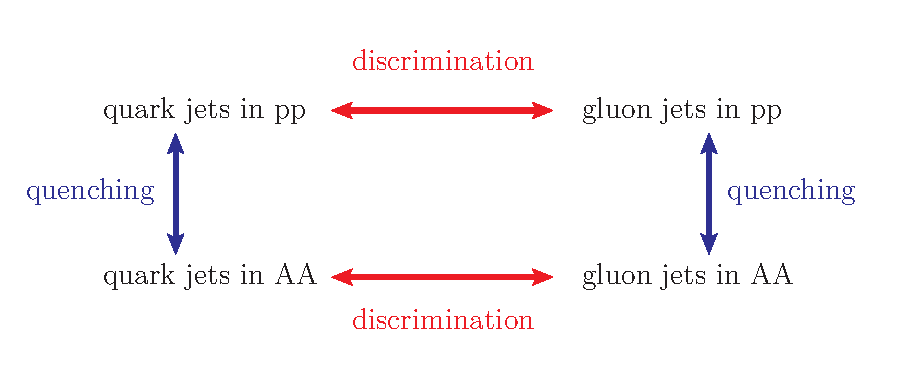
\includegraphics[width=0.6\textwidth]{plots/qg_HI}
	   \caption{Illustration of the interplay between jet quenching (vertical) and quark gluon discrimination (horizontal). }
	   \label{fig:quenching_discrimination}
\end{figure}

We will use quark jets and gluon jets as different probes of heavy ion collisions and compare their modification patterns. In doing so one attempts to identify jet features which are sensitive to aspects of quark and gluon jet quenching mechanisms. This can be quantified by studying the modification of specific jet substructure observables. Such direct approach is closely related to the outstanding problem of discriminating quark and gluon jets, where the goal is to exploit jet features which show differences between quark jets and gluon jets. One may compare quark jets and gluon jets in the same collision system and use their differences as a way to quantify the jet modification. This can help disentangle jet quenching effects on common features between quark and gluon jets and cancel systematic uncertainties in experiments. A schematic illustration of possible ways of exploiting quark and gluon jet substructure is shown in Fig:~\ref{fig:quenching_discrimination}.

Quark gluon discrimination has been studied extensively in the past\cite{}. With powerful tools for analyzing multiple variables, a large number of physics-motivated jet substructure observables have been examined systematically to identify the most useful ones \cite{Gallicchio:2011xq,Gallicchio:2012ez}. On the other hand, using modern machine learning image recognition techniques to process the raw input of the angular distribution of jet energy as jet images \cite{Komiske:2016rsd}, the discrimination performance can be significantly increased. This suggests that additional jet features have been identified by the deep neural network to help the tagging task. We use both methods to gain insights on how jet quenching is manifested in these two jet representations. Furthermore, we develop the telescoping deconstruction framework which represents the whole jet information using subjets with different angular resolution. It introduces an organization in the decomposition of jet substructure which allows order-by-order examination of jet features. The details about telescoping deconstruction are provided in Appendix.

\subsection{Physics-motivated Multivariate Analysis}
\label{sec:mva}

\begin{figure}[h]
	   \centering
	   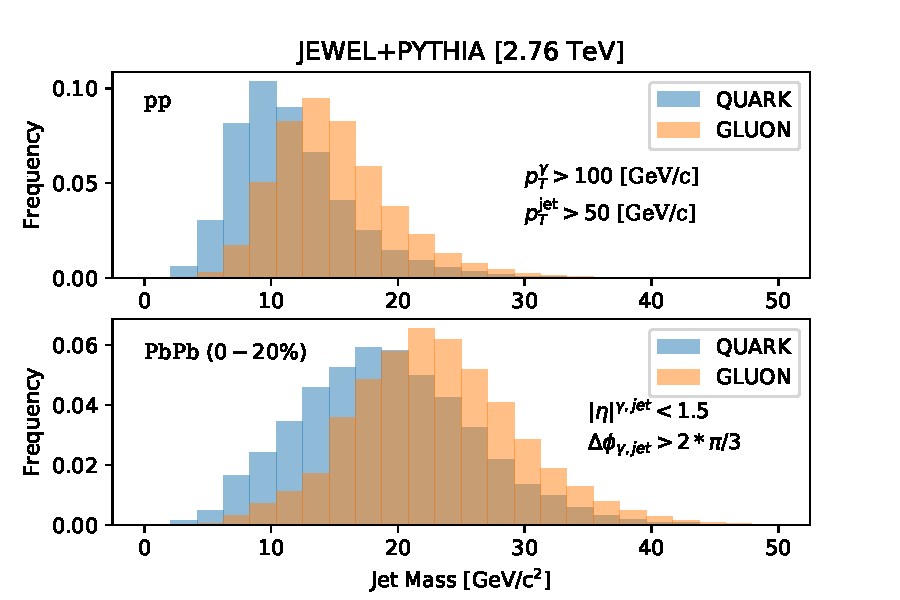
\includegraphics[width=0.48\textwidth]{plots/JEWEL_pp_pbpb020_jetMass}
	   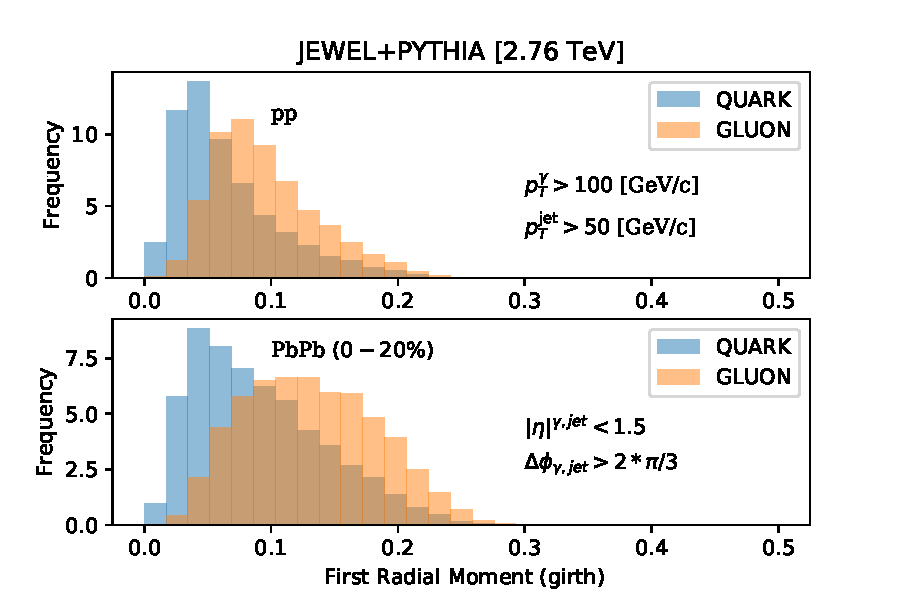
\includegraphics[width=0.48\textwidth]{plots/JEWEL_pp_pbpb020_firstRadialMoment}
	   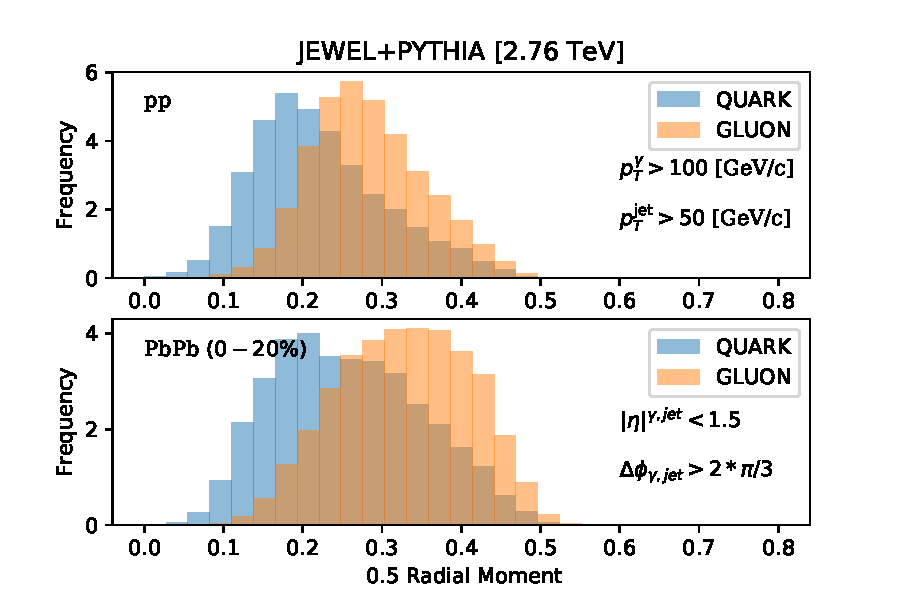
\includegraphics[width=0.48\textwidth]{plots/JEWEL_pp_pbpb020_halfRadialMoment}
	   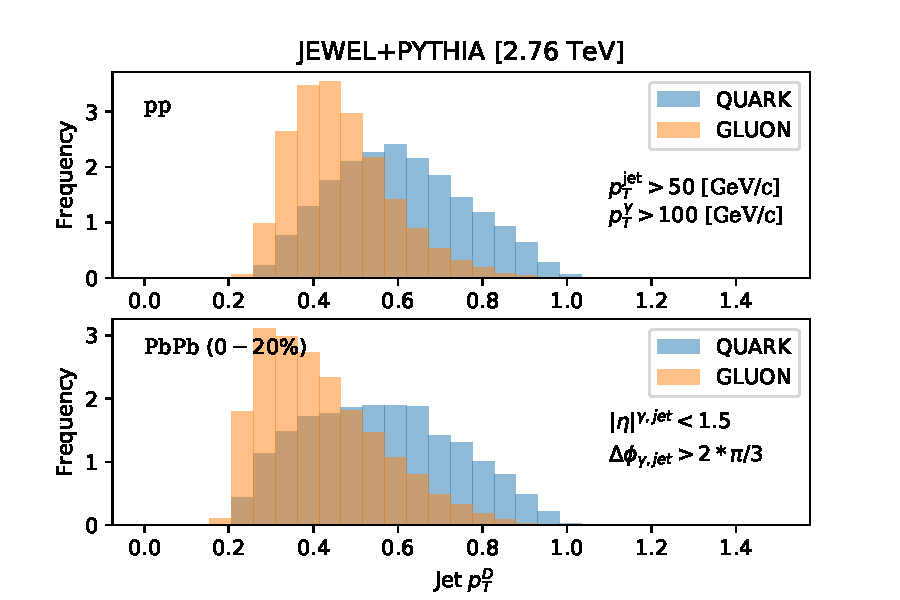
\includegraphics[width=0.48\textwidth]{plots/JEWEL_pp_pbpb020_pTD}
	   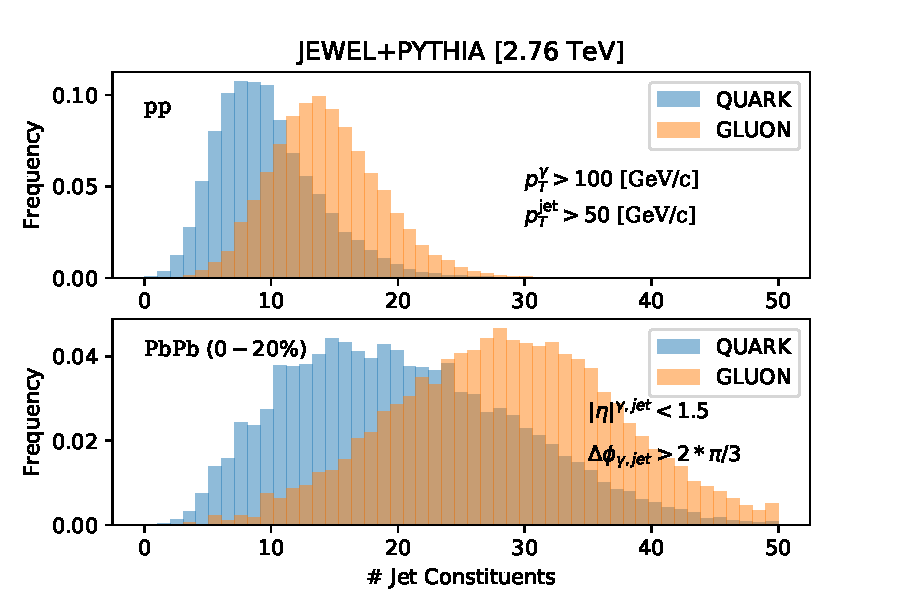
\includegraphics[width=0.48\textwidth]{plots/JEWEL_pp_pbpb020_NumberjetConstituents}
	   \caption{Distributions of the jet constituents (top left), invariant jet mass (top right), $p^{D}_{T}$ (center left), the half radial moment (center right) and the jet girth or the first radial moment (bottom) for quark (darker blue) and gluon (lighter orange) induced jets (color online). The top panels of each individual distribution show the pp and the bottom panels correspond to central (0-20\%) PbPb events generated by the \jw generator.}
	   \label{fig:jetdistributons_pp_pbpb}
	\end{figure}

Multivariate analysis have been successfully employed in object classification and selection by the LHC experiments \cite{} and thus an effective, physics-motivated baseline in our study. Given a jet reconstructed using the anti-$k_{t}$ algorithm \cite{Cacciari:2008gp}, we choose the following set of five jet substructure observables \cite{} to highlight the differences in quark jets and gluon jets,
	\begin{itemize}
		\item Jet mass: $m = \sqrt{(\sum_{i\in {\rm jet}} p_i)^2}$. 
        \item First radial moment (girth): $\sum_{i \in {\rm jet}} p^i_{T} \Delta R_{{\rm jet}, i}/p^{\rm jet}_{T}$, where $\Delta R_{{\rm jet}, i}=\sqrt{\Delta \eta^2_{{\rm jet}, i}+\phi^2_{{\rm jet}, i}}$.
		\item 0.5 radial moment:  $\sum_{i \in {\rm jet}} p^i_{T} (\Delta R_{{\rm jet}, i})^{0.5}/p^{\rm jet}_{T}$.
        \item $p_{T}^{D}$: $p^{D}_{T} = \sqrt{\sum_{i \in {\rm jet}} {p^{i}_{T}}^2}/p^{\rm jet}_{T}$.
        \item Pixel multiplicity: the number of $(\eta,\phi)$ pixels with energy deposit. %including charged and neutral; given by the anti-k$_{t}$ algorithm
	\end{itemize}

Fig:~\ref{fig:jetdistributons_pp_pbpb} shows the distributions of the above jet observables in pp and PbPb collisions. The quark and gluon jets used in plotting Fig:~\ref{fig:jetdistributons_pp_pbpb} include the grid dicretization. Furthermore, jets in PbPb collisions are subtracted using the GridSub background subtraction method. Note that the jet mass and radial moments are infrared and collinear (IRC) safe observables with different weights on the particle angular distributions. In vacuum, they reflect the fact that gluon jets have larger jet mass and radial moments than quark jets due to the larger color charge and Casimir color factor $C_A>C_F$. In the \jwpy-simulated PbPb collisions, for both quark and gluon jets the distributions are consistently modified towards larger values. On the other hand, $p_T^D$ and the pixel multiplicity are IRC unsafe. We see that there is significant increase of the pixel multiplicity and decrease of the values of $p_T^D$. This is due to the presence of the increased number of soft particles inside jets from the \jw ~medium recoil contributions \cite{}.

It is important to note that these observables are sensitive to the jet clustering algorithm, the minimum \pt ~cutoff of jet constituents and the background subtraction procedures employed. In order to facilitate a direct comparison between experimental data and Monte Carlo simulations, one has to either unfold the detector resolution from these observables or perform Monte Carlo simulations with detector response. The unfolding procedure for jet observables increases in dimensionality and complexity as the correlations among observables become strong. For example, the jet mass will have to be unfolded in the 4-dimensional distribution of the generated and reconstructed jet \pt ~and mass.

We combine the five jet substructure observables using a multivariate model implemented in Keras, with two dense layers of 10 nodes each. We use the rectified linear unit (\textit{relu}) and sigmoid activation functions for the dense layers and the output layer, respectively. The model training utilizes the Adam optimizer and the binary cross entropy loss function. We perform cross validation using Monte Carlo samples which are split into two halves for training and testing.

%All five jet observables showcase the ability to classify quarks vs gluons in both pp and PbPb. Recent results from LHC experiments on the effect of jet quenching on inclusive jets showcase two main features; a slight narrowing of the jet core and increased low \pt particle multiplicity in the periphery regions of the jet leading to a broadening of the jet shape. Such an effect is captured in \jw, with the introduction of the medium induced recoils and introduces a further complexity in the question of quark vs gluon classification in PbPb. In vacuum, we expect gluon jets to be broader than quark jets due to the different in the casimir color factor and thus in PbPb collisions, with both jets being quenched and broader, the ability to discriminate effectively between quark and gluon jets is expected to reduce when one only considers fragmentation based observables as we proceed to show in the upcoming sections.

\subsection{Jet Image}
\label{sec:image}

\begin{figure}[t]
\centering
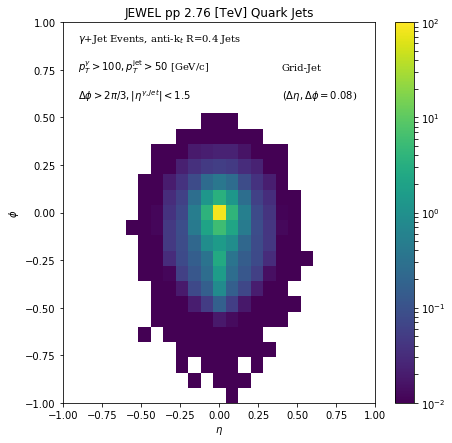
\includegraphics[width=0.45\textwidth]{plots/jewel_pp_avgQuarkJet}
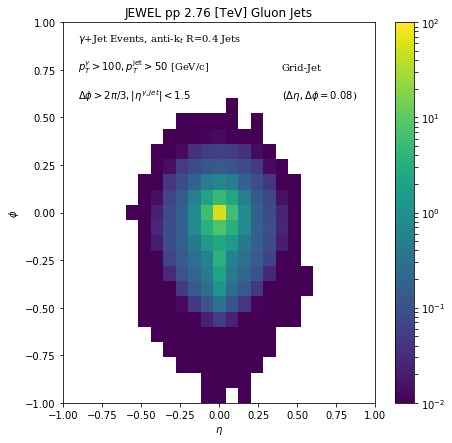
\includegraphics[width=0.45\textwidth]{plots/jewel_pp_avgGluonJet}
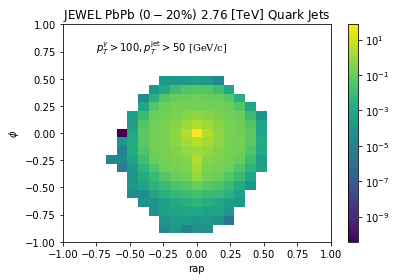
\includegraphics[width=0.45\textwidth]{plots/jewel_pbpb020_avgQuarkJet}
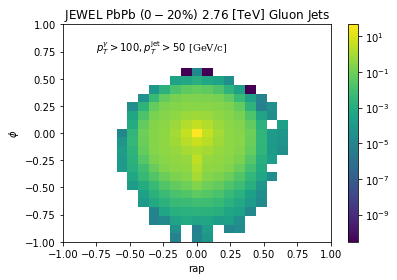
\includegraphics[width=0.45\textwidth]{plots/jewel_pbpb020_avgGluonJet}
\caption{Average quark (left) and gluon (right) pre-processed jet images shown in the $\eta-\phi$ plane for pp (top) and central PbPb (bottom) collisions generated from \jw. The color scale in the z axis represents the average pixel \pt in units of GeV/c. }
\label{fig:qgjetimages}
\end{figure}

The multivariate analysis discussed previously is a constructive approach to collect and examine the usefulness of jet features which may help distinguish quark jets from gluon jets. An alternative approach is to use image recognition techniques which optimize comprehensive multivariate models and identify all possible, useful features. The radiation pattern of a jet can be quantified as an image in the $\eta-\phi$ plane of transverse momentum deposit in detector calorimeter cells, much like a digital camera. The jet image thus represents a fixed-dimensional representation of jets. Each jet image is pre-processed \cite{deOliveira:2015xxd} by translating in $\eta$ and $\phi$ plane so that the highest pixel centers at the origin. Also, the image is rotated so that the principal component of the energy density is along the $\eta=0, \phi<0$ direction. 
 
Fig:~\ref{fig:qgjetimages} shows the average quark (left) and gluon (right) jet images in pp (top) and central PbPb (bottom) collisions. The color of each image pixel represents the transverse momentum deposited in the pixel. We see the broader energy distribution around the center pixel for gluon jets compared to quark jets in pp collisions, and the significantly broader distributions for jets in PbPb collisions. Note that in experiment it may be very challenging to directly analyze jet images due to detector and measurement considerations. Here we mainly use the jet image approach as a useful comparison of the classification performance.
	
A deep convolutional neural network implemented in Keras with the TensorFlow backend is utilized in this analysis. The neural network model consists of three convolution layers of sequentially reducing sizes, each with 8 filters followed by a max-pooling layer. The convolution layers use hyperbolic tangent activation function, and the output layer uses sigmoid activation function. The output layer is preceded by three layers, a dropout layer with a rejection score of 0.20, a dense layer with 20 nodes and an additional dropout layer with a reduced rejection score of 0.10. The additional dropout layer helps filtering less important features from previous layers and thus increases the speed and efficiency of the model training. The model is trained using the Adam optimizer with binary cross entropy loss function.
	
\subsection{Telescoping Deconstruction}
\label{sec:tjet}

\begin{figure}[t]
\centering
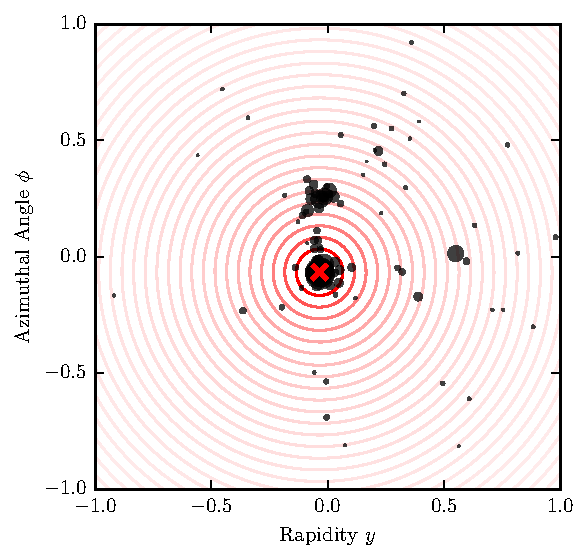
\includegraphics[width=.32\columnwidth]{figures/QCDjetT1_telescoped2.pdf}
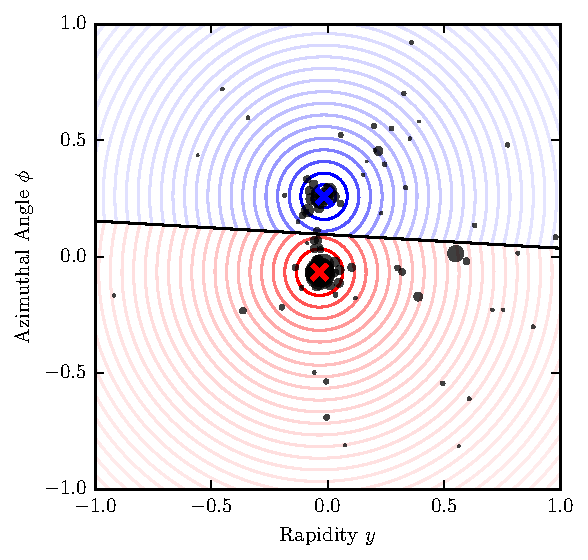
\includegraphics[width=.32\columnwidth]{figures/QCDjetT2_telescoped2.pdf}
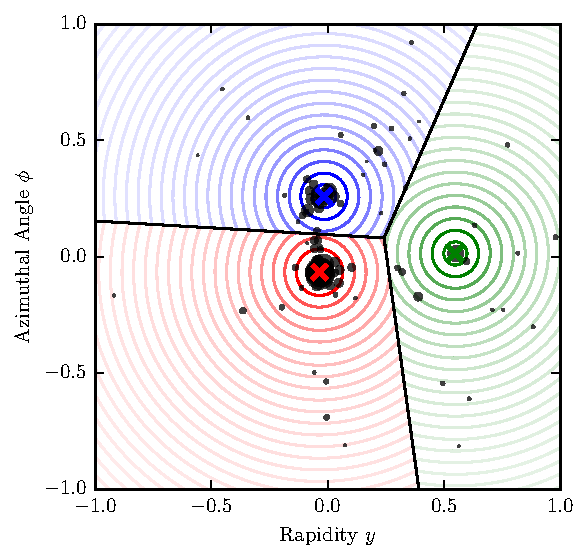
\includegraphics[width=.32\columnwidth]{figures/QCDjetT3_telescoped2.pdf}
\caption{Illustration of telescoping deconstruction at T1 (left panel), T2 (middle panel) and T3 (right panel) orders for a QCD jet. The crosses are the Winner-Take-All $k_T$ axes. The straight lines are the exclusive subjet boundaries. Particles are sized according to their transverse momenta. See Appendix for more details about the procedures.}
\label{fig:tjetQCD}
\end{figure}

The multivariate analysis and jet image recognition discussed previously are two characteristically different methods. The multivariate analysis uses physics-motivated observables and is a ``bottom-up" approach to collect useful jet features. However, the set of observables identified may be highly correlated, and it is not clear how to systematically improve the method. On the other hand, jet images represent low-level, comprehensive jet information. The training of a deep neural network is a ``top-down" approach to identify all the useful features through the model optimization. However, extracting physical messages from the trained neural network parameters can be a challenging task.

We develop and apply the telescoping deconstruction (TD) framework in our study of quark and gluon jet substructures in pp and PbPb collisions. Telescoping deconstruction aims to embrace both advantages of multivariate analysis and jet image recognition. It decomposes jets using physics-motivated, comprehensive sets of observables which form an organized basis of jet substructures. It is a complete and systematic subjet expansion consisting simply of subjet kinematic variables. The expansion is ordered by $N$, the number of subjets exclusively reconstructed, and the individual telescoping deconstruction observables are physically-meaningful which encode the hard splitting of jets and non-perturbative physics. The telescoping procedure probes radiation around dominant energy flows in a jet with multiple angular resolutions. It efficiently quantifies the radiation distribution by first capturing the dominant energy in the subjet reconstruction and then reaching out to include wide-angle, soft radiation. Fig:~\ref{fig:tjetQCD} illustrates the telescoping deconstruction of a QCD jet at T1, T2 and T3 orders. The details about the telescoping deconstruction procedures are provided in Appendix, including the applications on boosted $W$ and top tagging in high energy physics.

For $R=0.4$ jets, we telescope around the subjets axes using radii from 0.08 to 0.4 with steps of 0.08. The subjet observables up to the $N$-th order are combined using dense neural networks to maximize the classification performance. We consider $N=\{1,2,3\}$ and the performance quickly saturates at $N=3$. {\bf add some ML details}

Beside the overall quark gluon classification performance using telescoping deconstruction, subjet variables within this framework can reveal many aspects of jet dynamics. In particular, there is rich information contained in subjet topology and subjet substructure. Recently, the CMS \cite{} and STAR \cite{} collaborations measured the groomed momentum sharing observable $z_g$. One reclusters jets using the Cambridge/Aachen algorithm \cite{Dokshitzer:1997in,Wobisch:1998wt} and sequentially removes wide angle, soft radiation until the following condition is satisfied by a branching,
\begin{equation}
    z_{\rm cut} < \frac{\min(p_{T_1},p_{T_2})}{p_{T_1}+p_{T_2}} \equiv z_g\;.
    \label{SD}
\end{equation}
Here $p_{T_1}$ and $p_{T_2}$ are the transverse momenta of the two branches, and $z_{\rm cut}$ is the soft-drop parameter which is set to $0.1$ in our analysis. Note that the Cambridge/Aachen clustering tree is angular-ordered, therefore the above procedure identifies the most wide angle, soft subjet which carries a significant fraction of the jet transverse momentum. The size of the soft subjet is dynamically determined and related to the angle $r_g$ between the two soft-drop branches, defined as the groomed jet radius. The observables $z_g$ and $r_g$ thus encode the kinematic information of the two subjets which is in the category of subjet topology. In vacuum, the observable $z_g$ is closely related to the Altarelli-Parisi splitting functions~\cite{Altarelli:1977zs}. The physical meaning of $z_g$ in heavy ion collisions have also been investigated \cite{Chien:2016led}. 

We use telescoping deconstruction to analyze the two soft-drop branches defining the $z_g$ observable. At the T2 order, we choose the subjet radius to be half the angle between the two deconstruction axes for subjet reconstruction. The distribution of the momentum fraction $z_{\rm T2}$ of the softer subjet is significantly different from the $z_g$ distribution, especially for gluon jets. Note that the axes used in the telescoping deconstruction procedure are defined with the Winner-Take-All scheme which favors energetic particles. We find that the axes at the T2 order may both align with the hard branch and are not able to efficiently tag the soft branch when it consists of soft particles. The situation is significantly improved at the T3 order where we use three axes to capture the soft branch in soft-drop. We combine two closest subjets, reducing the number of subjets to two, and the distributions of the momentum fraction $z_{\rm T3}$ of the softer subjet for quark and gluon jets are very similar. In comparison, we reconstruct subjets around the axes of the soft-drop branches to probe their energy distributions. We find that the distribution of the momentum fraction $z_{{\rm T2},g}$ of the softer subjet is very similar to that of $z_{\rm T3}$ and different from that of $z_g$. This suggests that the active areas of the two soft-drop branches are different. On the other hand, the subjet substructure may allow us to extract the information about the partonic origin of subjets. We look at the scaleless ratio $m_i/p_{T_i}$ where $m_i$ is the light (heavy) subjet mass, or the mass of the hard (soft) subjet.

\section{Quark and Gluon Jet Modification and Discrimination}
\label{sec:results}

We discussed jet representations using multiple physics-motivated variables, jet images and telescoping deconstruction. In this section we will use these information in the study of jet modification and quark gluon discrimination. For quark gluon discrimination, the performances are shown using Receiver Operating Characteristic (ROC) curves which plot the gluon jet efficiency as a function of the quark jet efficiency. We also perform discriminations between jets in pp and AA collisions for both quark jets and gluon jets, and the performance is evaluated by the ROC curves showing AA jet efficiency as a function of the pp jet efficiency. A lower ROC curve represents a better performance.

\begin{figure}
	   \centering
	   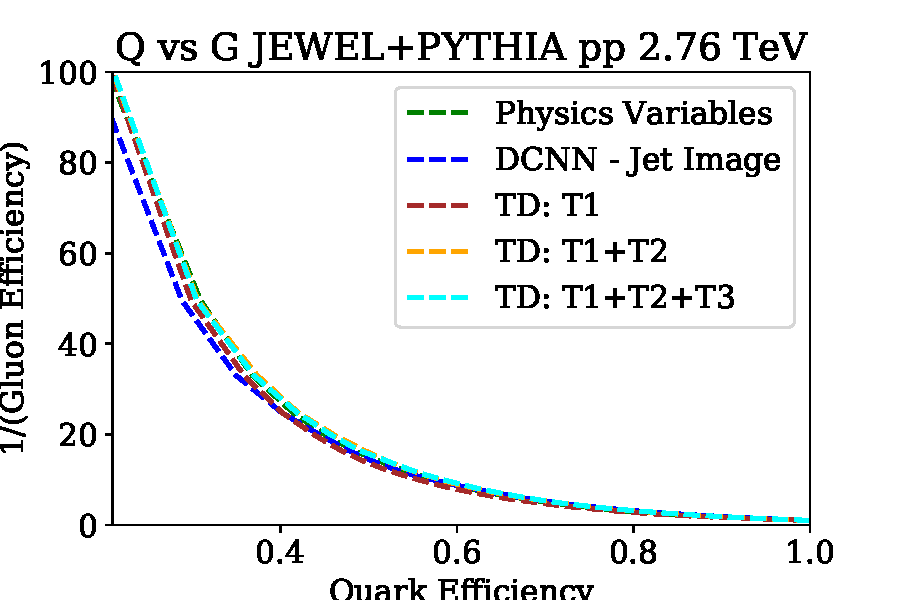
\includegraphics[width=0.49\textwidth]{plots/JEWELPYTHIA_pp_2p76TeV_genLevel_QvsG.pdf}
	   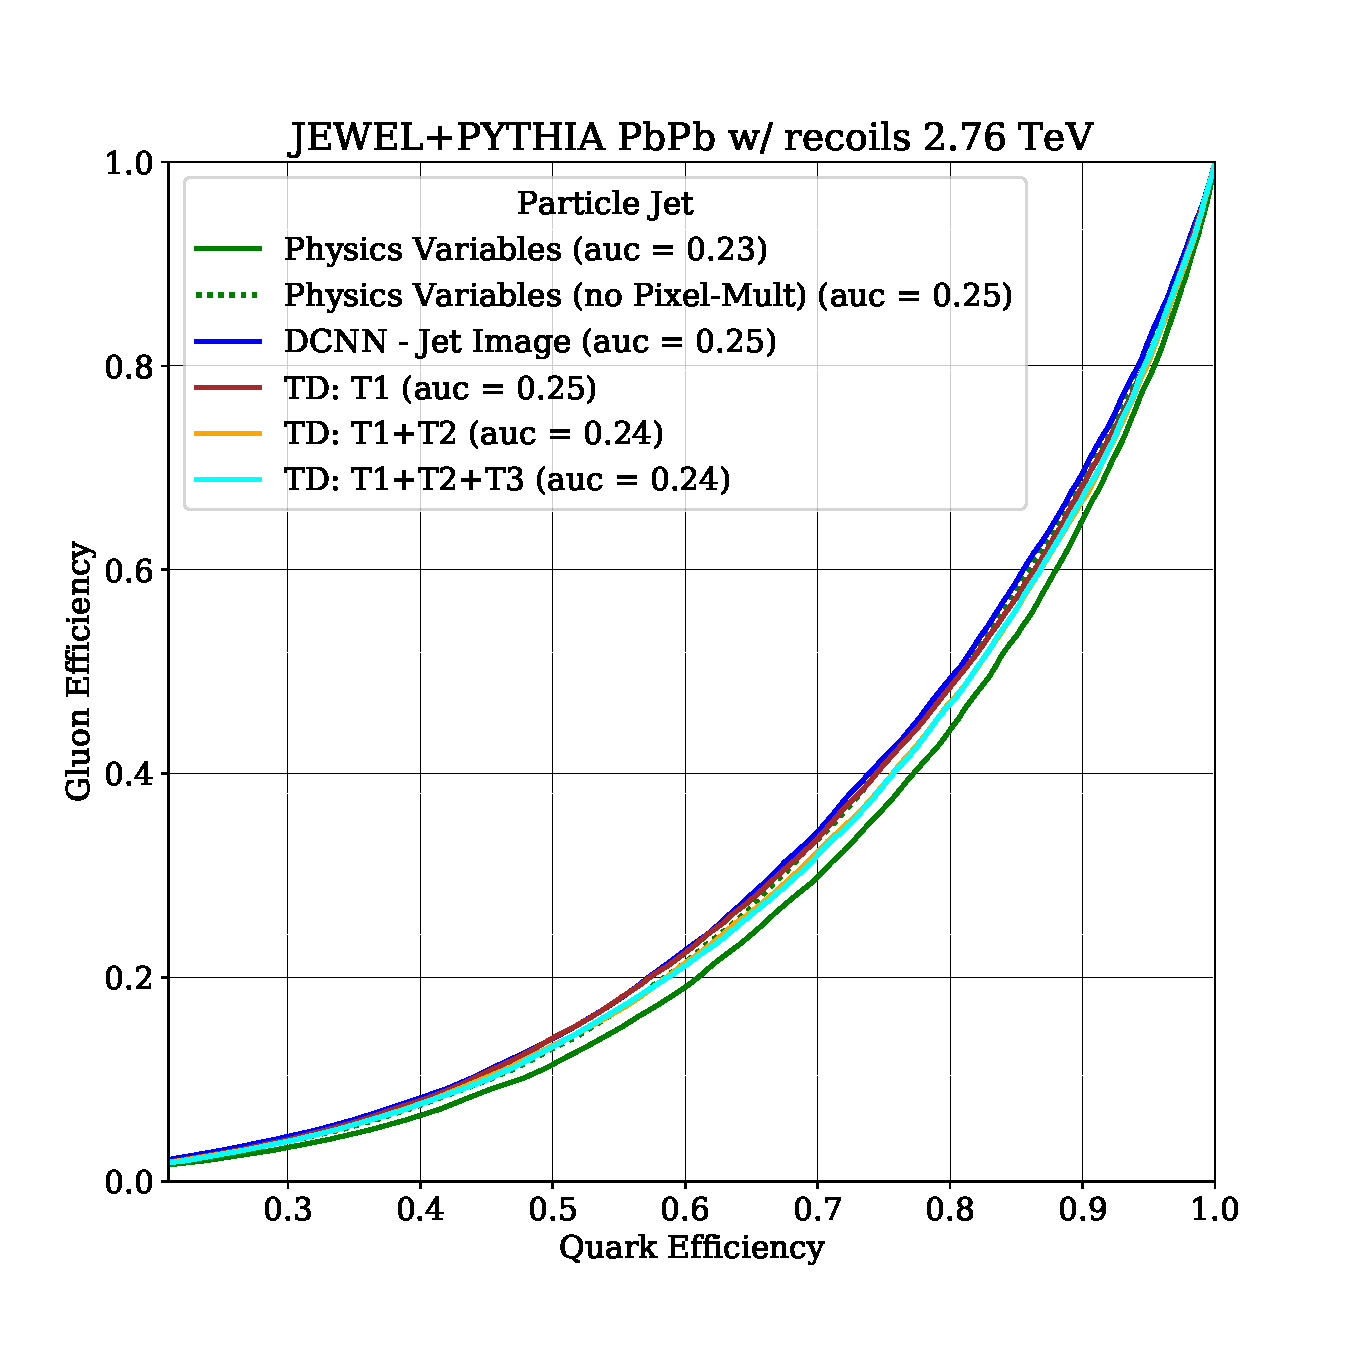
\includegraphics[width=0.49\textwidth]{plots/JEWELPYTHIA_PbPb_2p76TeV_genLevel_QvsG.pdf}
	   \caption{}
\label{fig:ROC_all}
\end{figure}

Fig:~\ref{fig:ROC_all} shows the ROC curves for quark gluon discrimination using physics-motivated variables, jet images and telescoping deconstruction in pp (left panel) and AA (right panel) collisions, using particle momenta when evaluating the observables without $\eta=\phi$ discretization and background subtraction. We see that overall the methods give similar performances, implying that the three jet representations capture sufficient jet information. Note that there is monotonic increase of the telescoping deconstruction performances from $\rm T1$ to $\rm T1+T2$ to $\rm T1+T2+T3$ with increasing input information of higher-order subleading subjets, and the performance saturates quickly at the T2 order. In the AA case, combining physics variables gives better performance due to the high particle multiplicity in the \jwpy-simulated AA events. Telescoping deconstruction with radius scan in steps of 0.08 is not able to capture the full multiplicity information at the T3 order.

\begin{figure}
	   \centering
       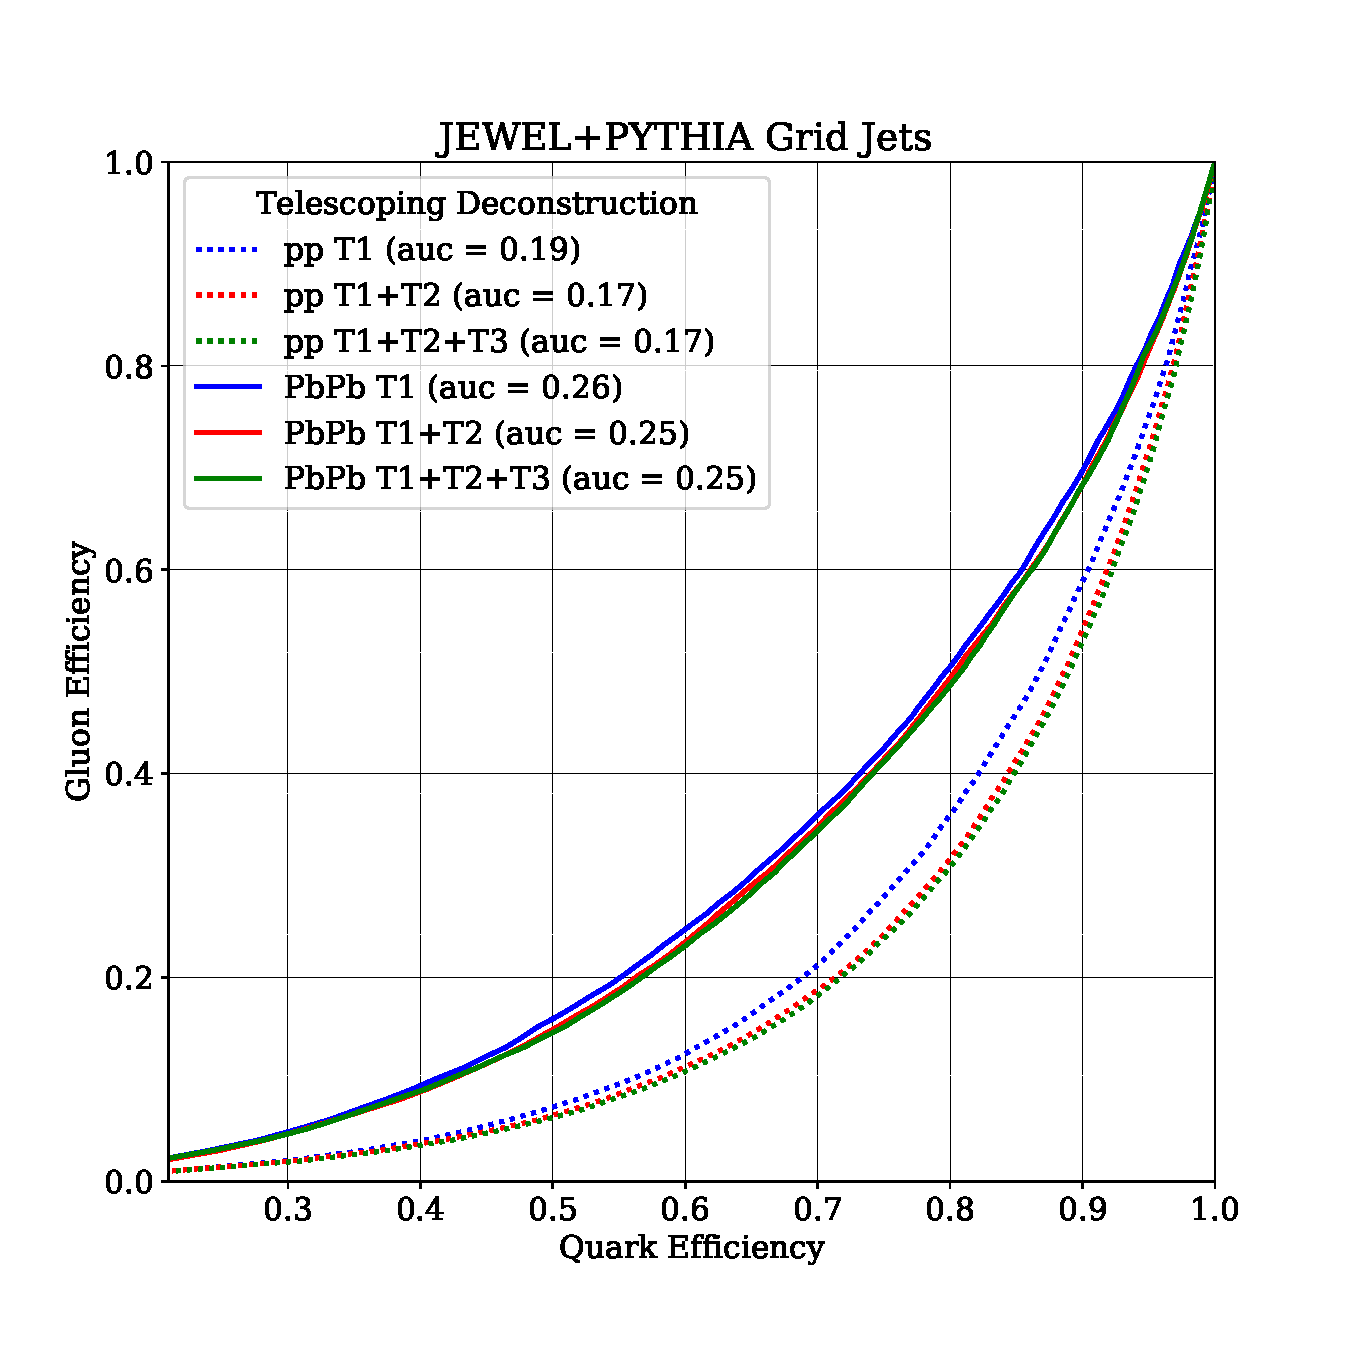
\includegraphics[width=0.49\textwidth]{plots/JEWELPYTHIA_TD_2p76TeV_ppvsPbPb.pdf}
       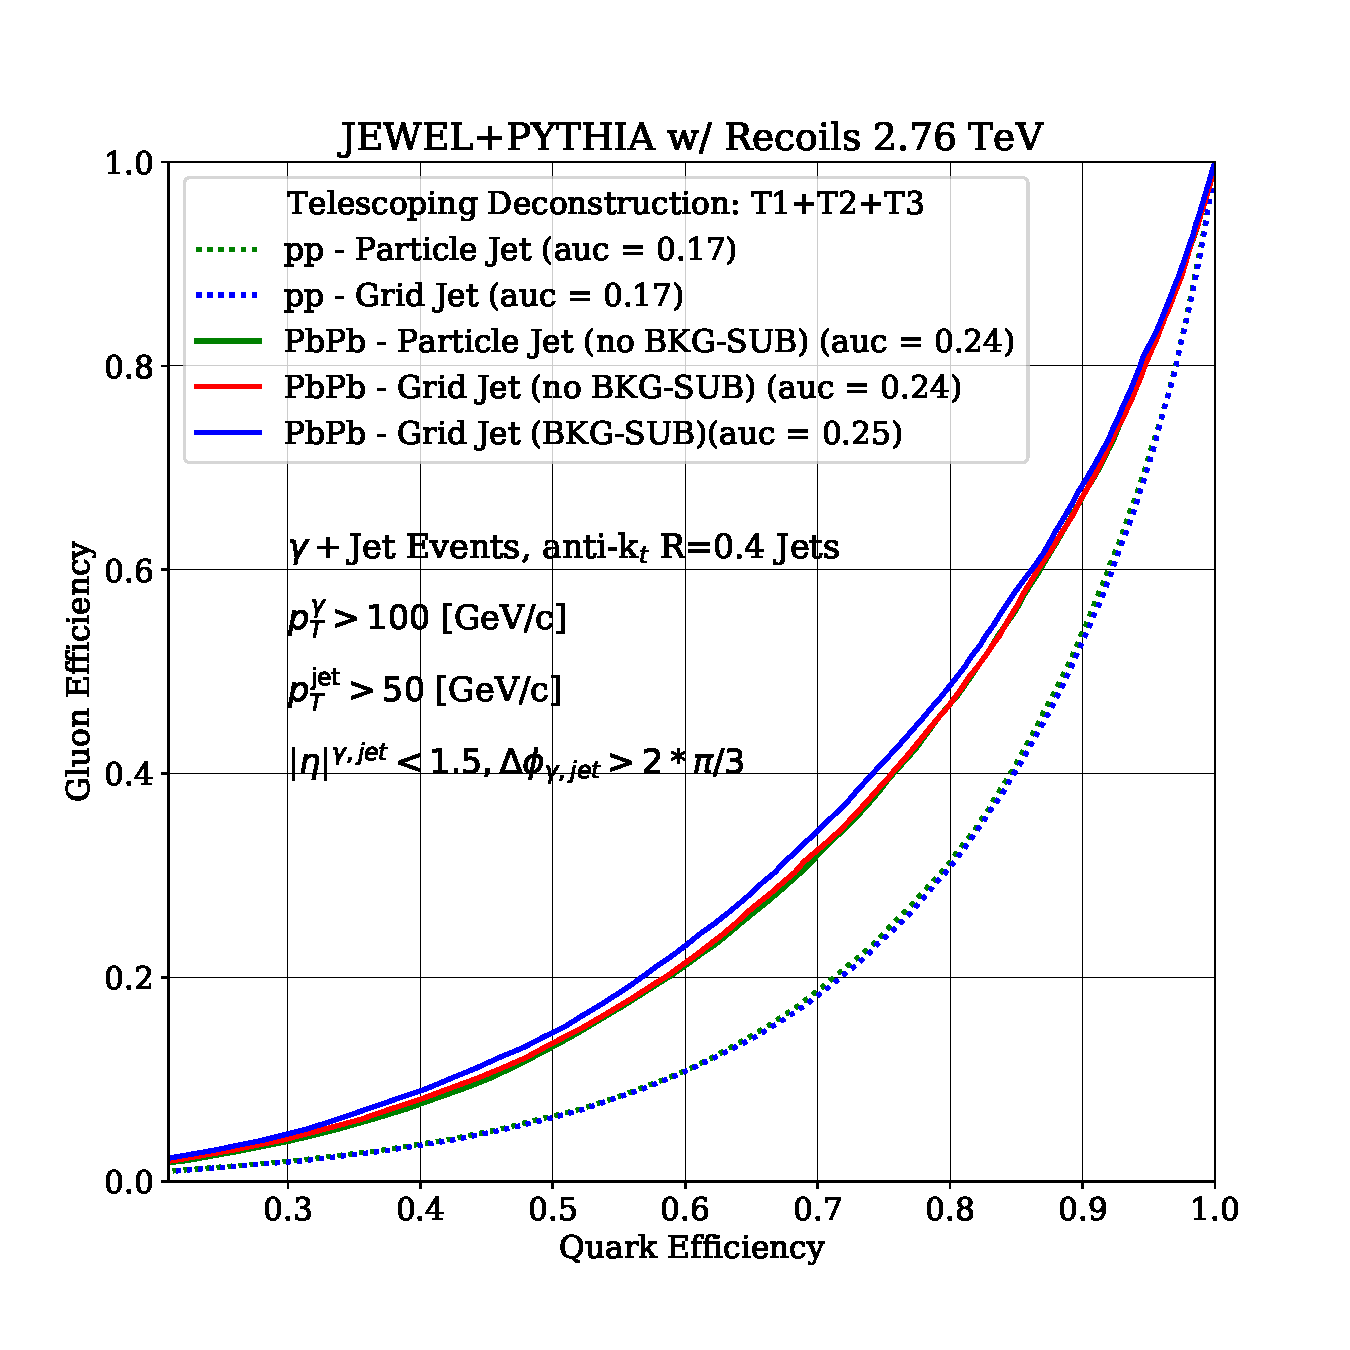
\includegraphics[width=0.49\textwidth]{plots/JEWELPYTHIA_TD123_2p76TeV_ppvsPbPb_comp_QvsG.pdf}
	   \caption{}
\label{fig:ROC_TD_input}
\end{figure}

By comparing the performances in pp and AA collisions, we clearly see that the performances drops in AA collisions. To have a closer look at the change of the classification performance from pp to AA collisions and the convergence of the TD performance, we plot the ROC curves of telescoping deconstruction in both pp and AA collisions in the left panel of Fig:~\ref{fig:ROC_TD_input}. We see the shrink of the performance improvement from T1 to $\rm T1+T2$ in AA collisions. This suggests that the information carried in higher-order subleading subjets can be washed out in heavy ion collisions due to the huge underlying-event soft activities or, more interestingly, the thermal randomization caused by the medium interactions in \jwpy. In the right panel of Fig:~\ref{fig:ROC_TD_input} we plot the TD ROC curves with different inputs with or without $\eta-\phi$ discretization and background subtraction. Since the radius scan in TD respects the $\eta-\phi$ discretization resolution, we don't see the change of the TD performance. On the other hand, the performance drops with the background subtraction performed. This suggests that some intrinsic differences between quark jets and gluon jets are removed in the subtraction. 

\begin{figure}
	   \centering
	   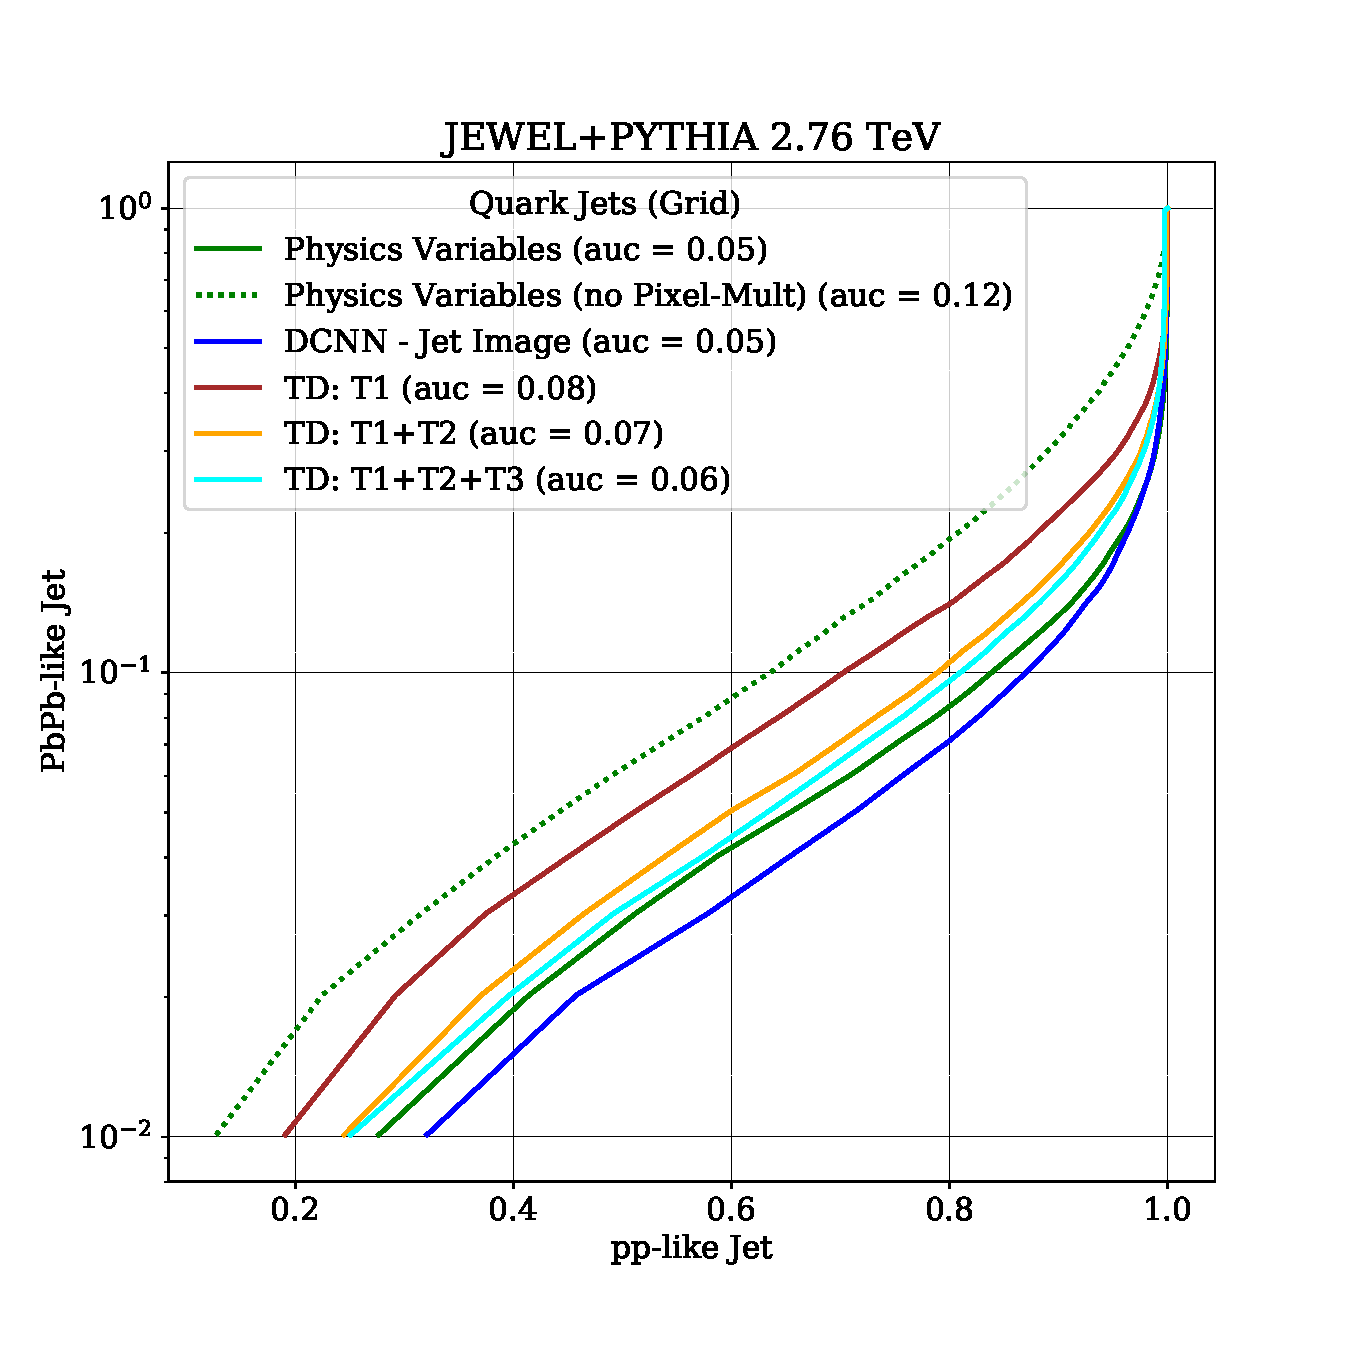
\includegraphics[width=0.49\textwidth]{plots/JEWELPYTHIA_2p76TeV_quark_ppvspbpb.pdf}
	   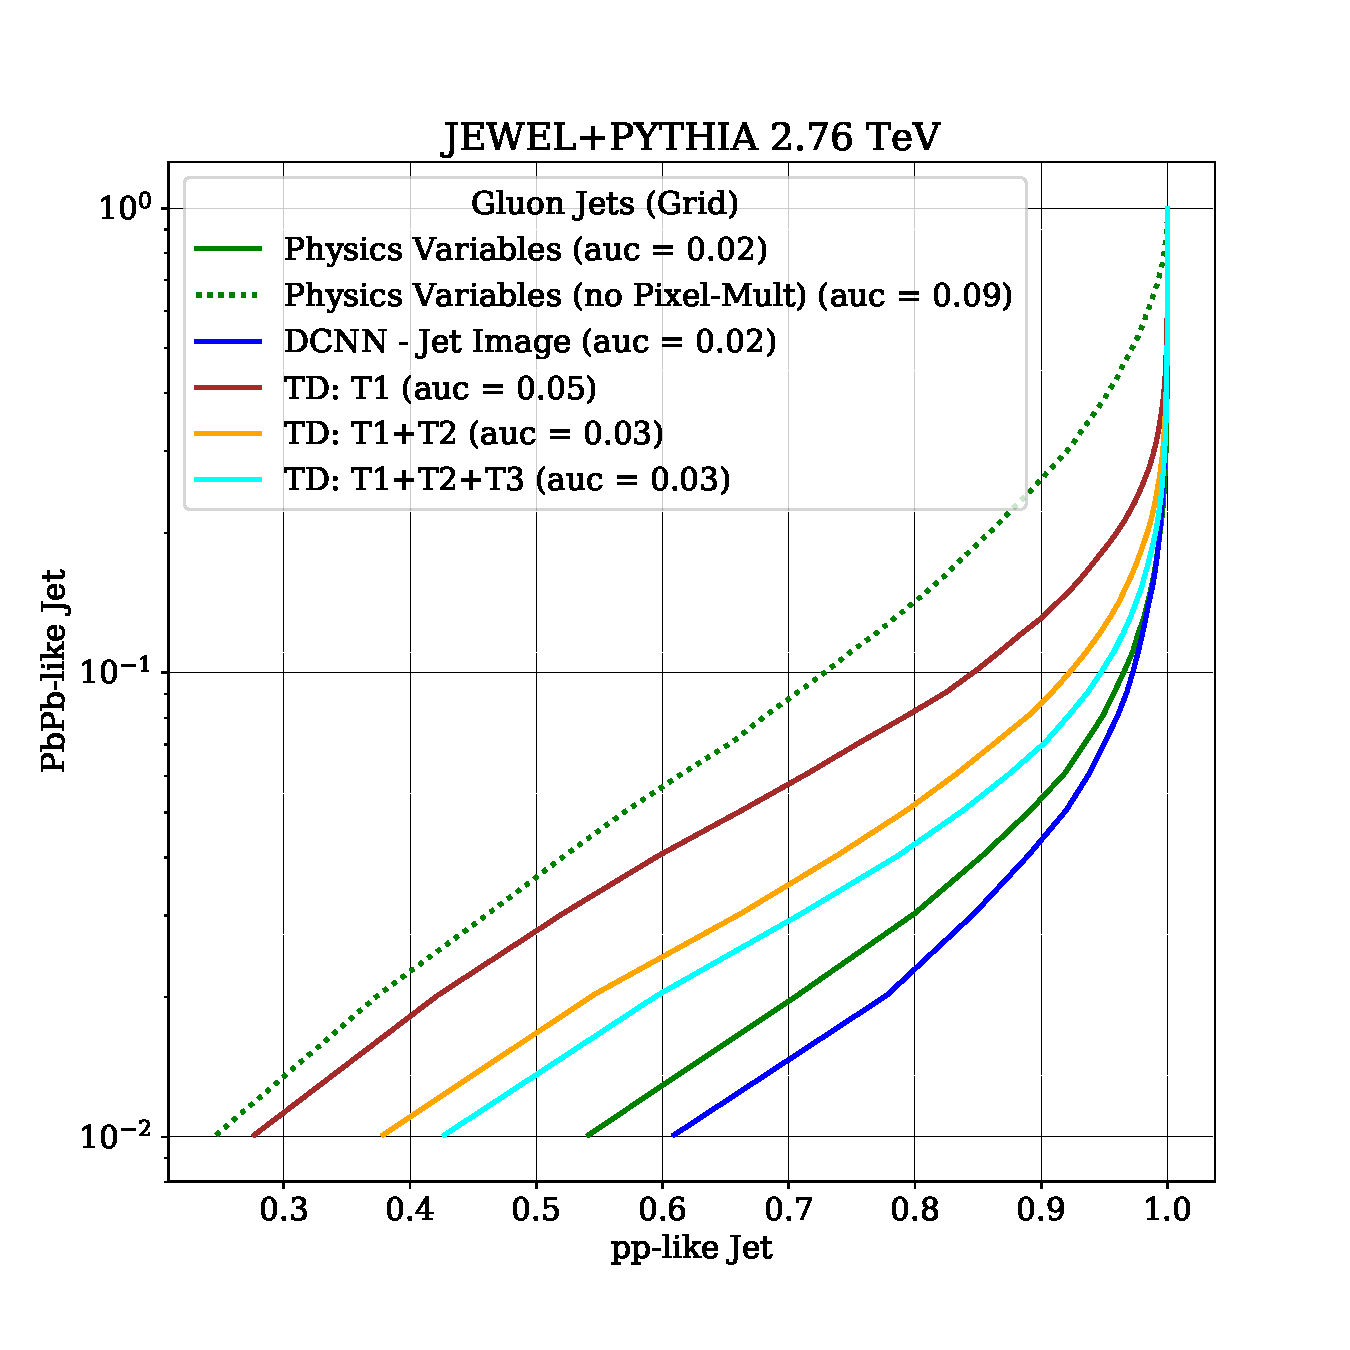
\includegraphics[width=0.49\textwidth]{plots/JEWELPYTHIA_2p76TeV_gluon_ppvspbpb.pdf}
	   \caption{}
\label{fig:ROC_qq_gg}
\end{figure}
Fig:~\ref{fig:ROC_all} shows the ROC curves for discriminating quark jets (left panel) and gluon jets (right panel) in pp and AA collisions using physics-motivated variables, jet images and telescoping deconstruction. We see huge difference between jets in pp and AA collisions therefore we plot the ROC curve using log scale in the y-axis. The significantly better performance in the gluon jet discrimination suggests that the modification of gluon jets is larger. We observe that the increase of the pixel multiplicity is a key feature in jet modification.

\section{Quark and Gluon Jets in Lund Diagrams}
\label{sec:lund}

\begin{figure}
	   \centering
	   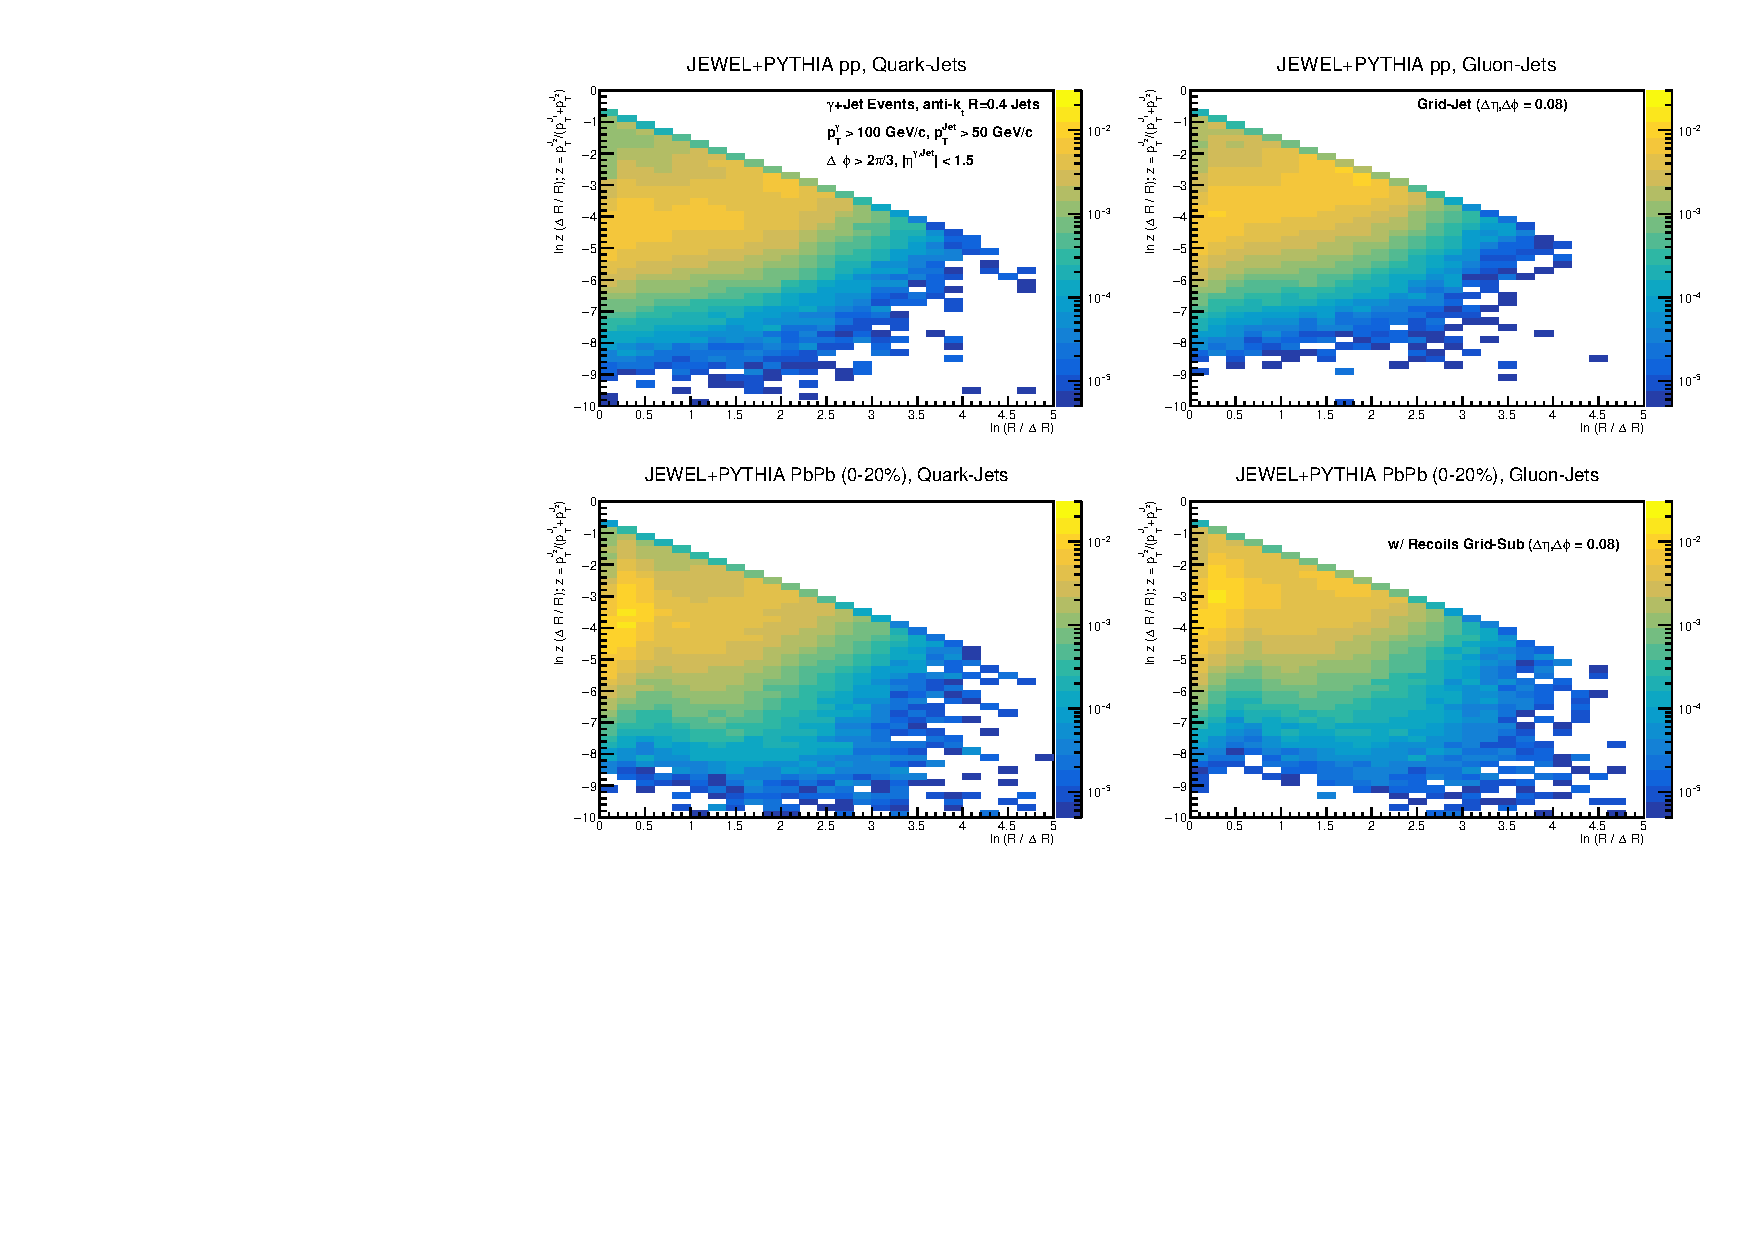
\includegraphics[width=0.9\textwidth]{plots/Individual_LundDiagrams_zrel.pdf}
	   \caption{}
\label{fig:Lund_full}
\end{figure}
Fig:~\ref{fig:Lund_full} shows the Lund diagrams for quark jets (left) and gluon jets (right) in pp (top) and AA (bottom) collisions. Note that only the splitting in the soft-drop hard branch enter into the Lund diagrams. We see the significant contributions from soft, wide-angle radiation in AA collisions.

\begin{figure}
	   \centering
	   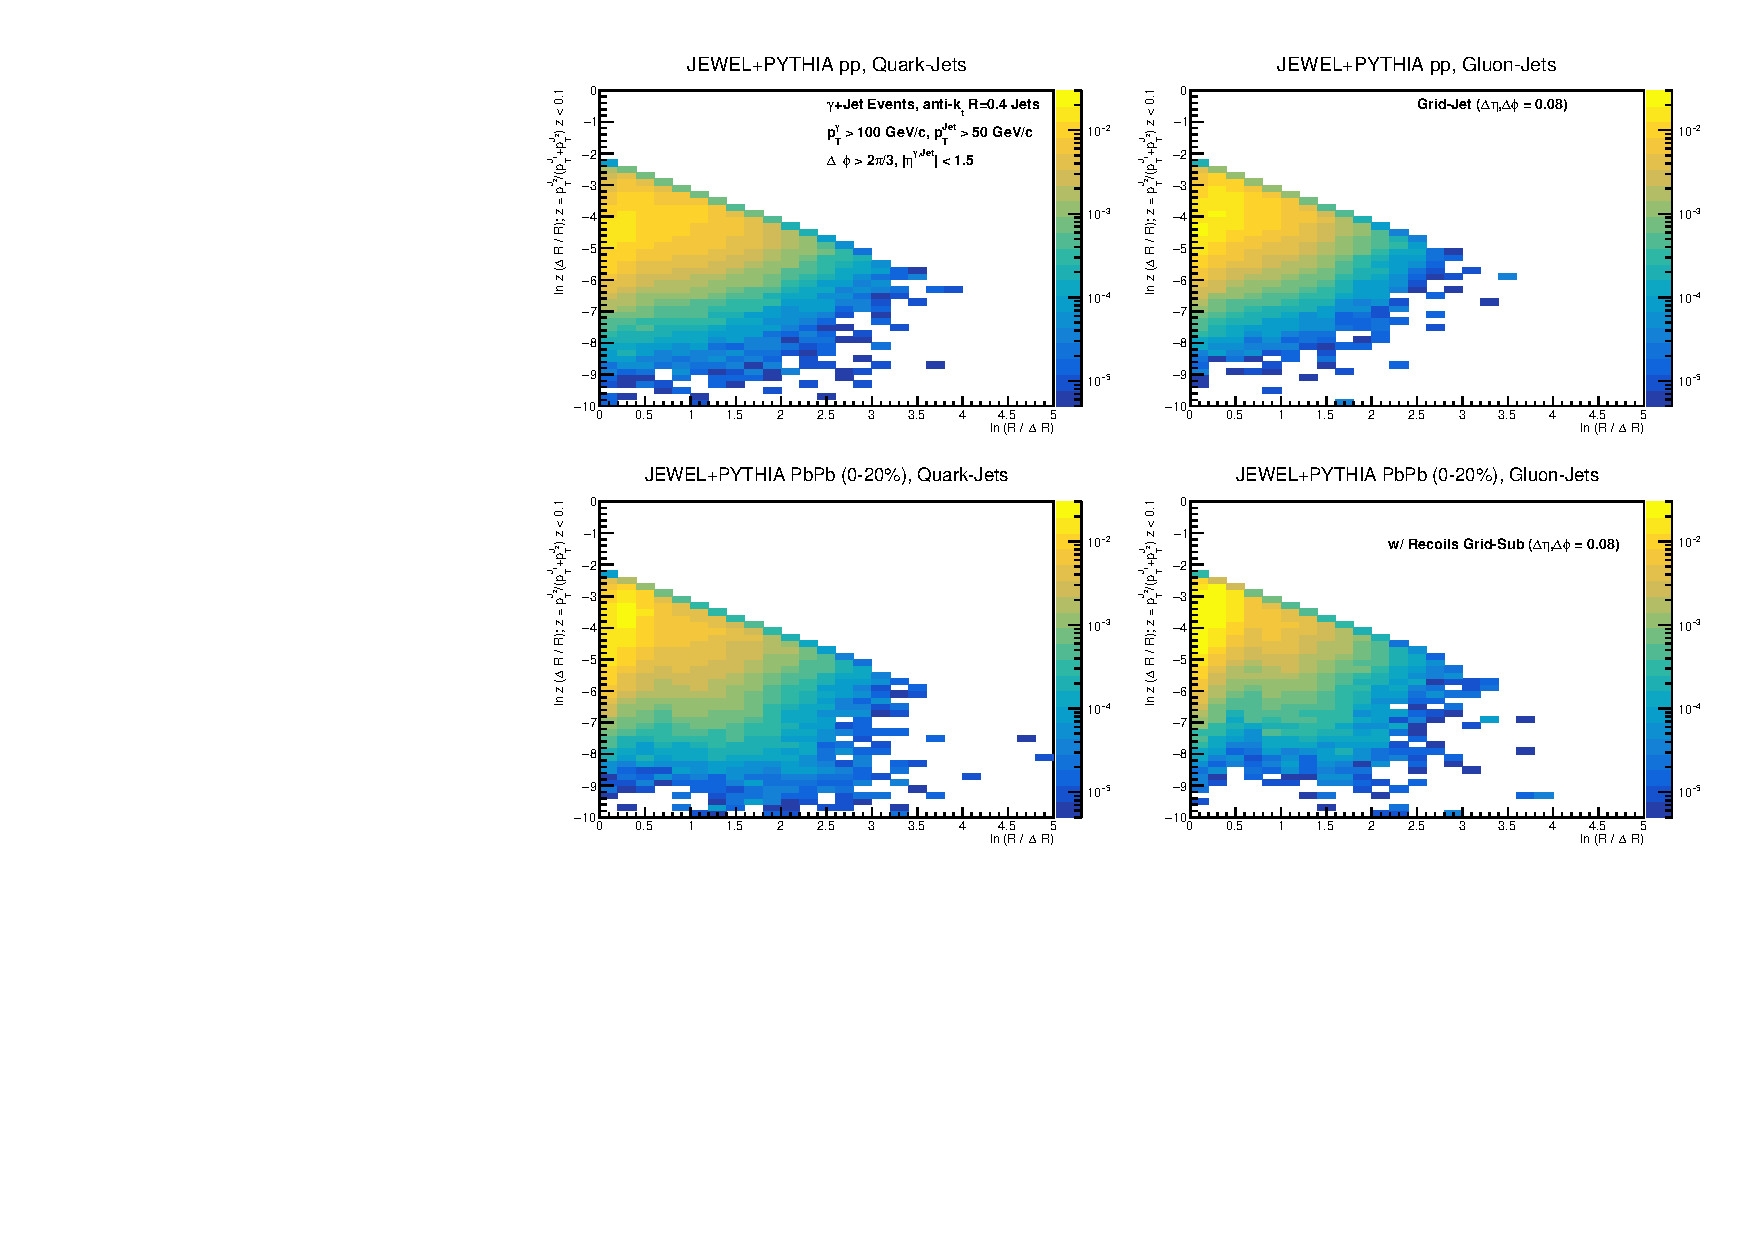
\includegraphics[width=0.9\textwidth]{plots/Individual_LundDiagrams_zrel_background.pdf}
	   \caption{}
\label{fig:Lund_bkg}
\end{figure}
Fig:~\ref{fig:Lund_bkg} shows the Lund diagrams for C/A trees before the one which passes the soft-drop condition. We see that the soft, wide-angle radiation is isolated. 

\begin{figure}
	   \centering
	   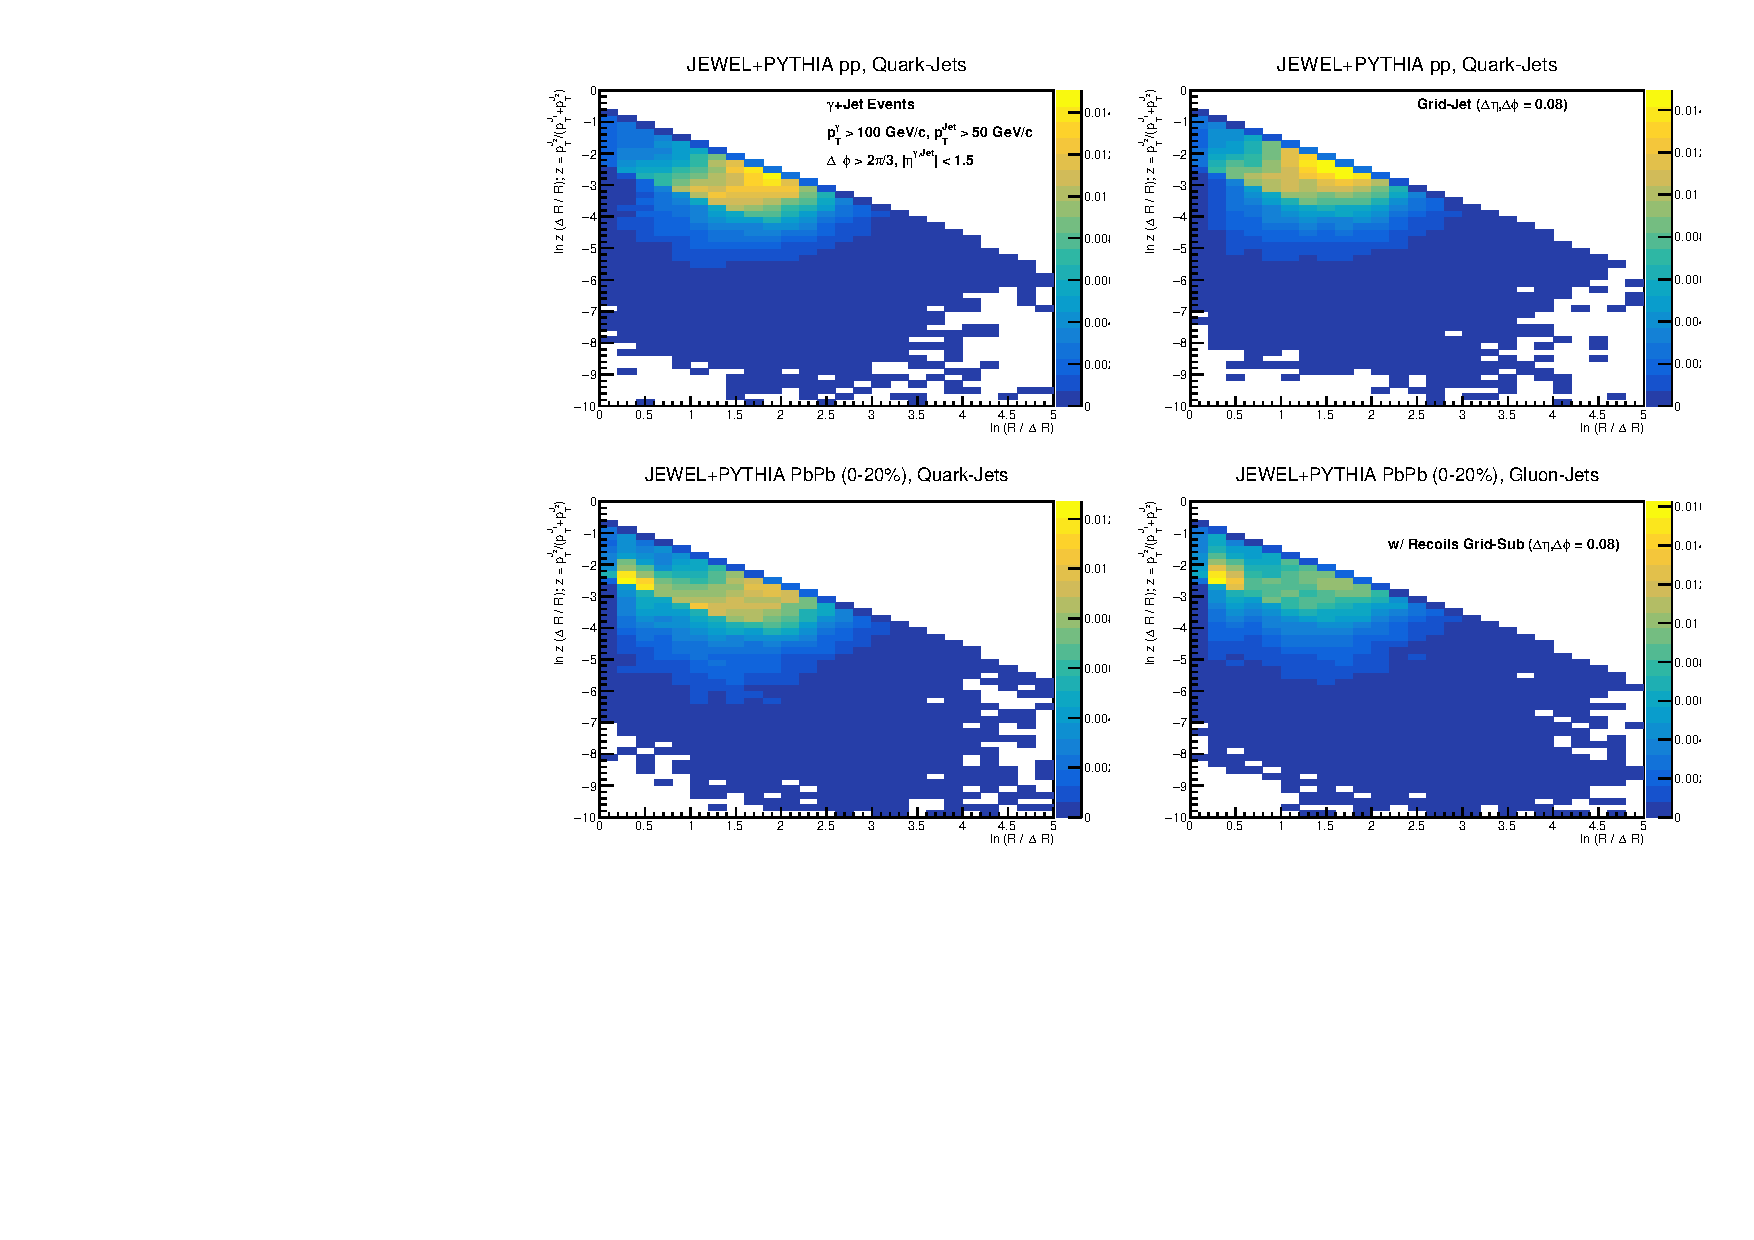
\includegraphics[width=0.9\textwidth]{plots/Individual_LundDiagrams_zrel_hardBranch.pdf}
	   \caption{}
\label{fig:Lund_hard}
\end{figure}
Fig:~\ref{fig:Lund_hard} shows the Lund diagrams for C/A trees after the hard branch in soft-drop. We see that the vacuum structure starts to emerge in the soft-drop AA jets. However, soft-drop can not remove all the soft radiation within the hard branch in AA collisions.

\begin{figure}
	   \centering
	   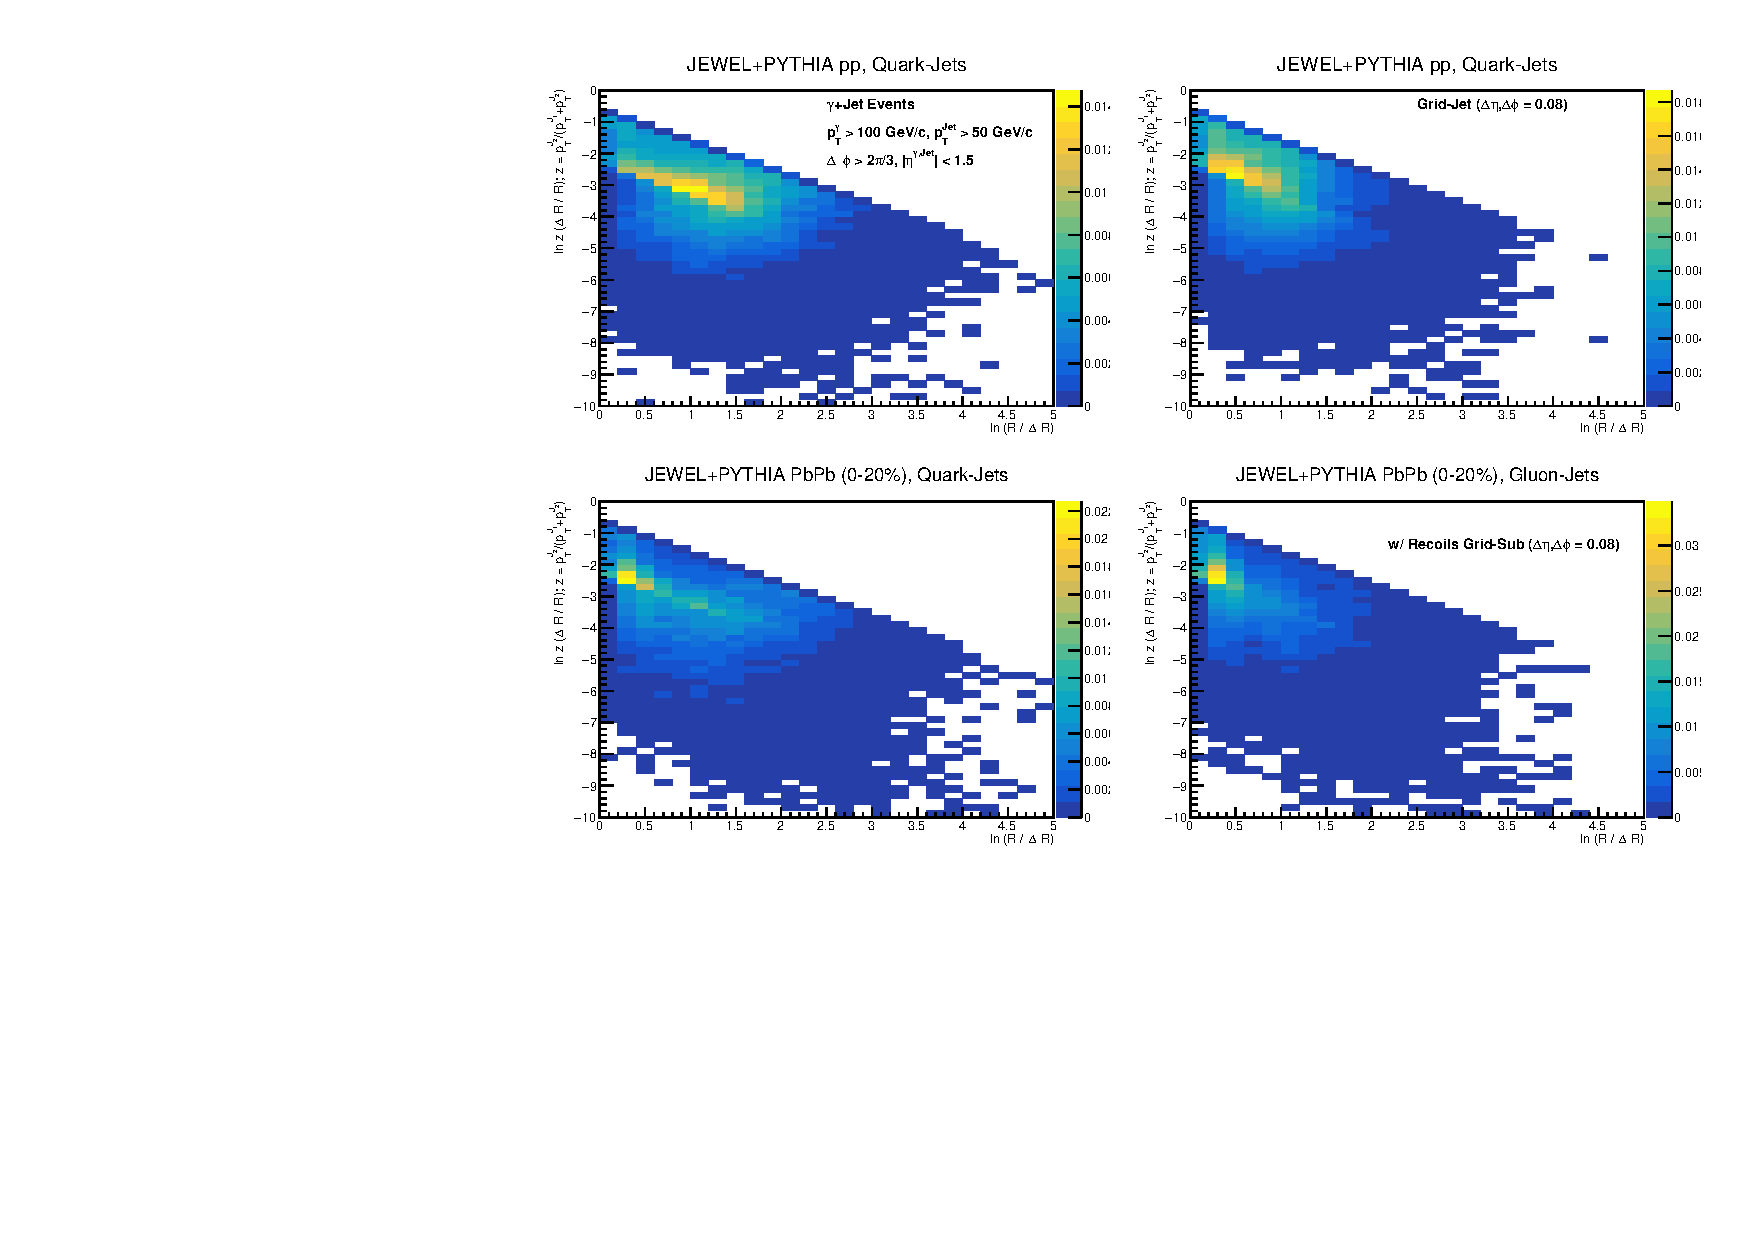
\includegraphics[width=0.9\textwidth]{plots/Individual_LundDiagrams_zrel_zgrg.pdf}
	   \caption{}
\label{fig:Lund_zgrg}
\end{figure}


\section{Conclusions}
\label{sec:conc}


\section*{Acknowledgments}
The authors are grateful to Patrick Komiske and Eric Metodiev for collaborating on the development of telescoping deconstruction and contributing to Appendix. The authors also thank Benjamin Nachman and Sevil Salur for helpful discussions, and . Y.-T. Chien was supported by the LHC Theory Initiative Postdoctoral Fellowship under the National Science Foundation grant PHY-1419008. R.K. Elayavalli acknowledges support from the National Science Foundation under Grant No.1067907 \& 1352081 (+JETSCAPE?).

























\newpage
\appendix
\section*{Appendix}
\section{Probing subjet energy flows with telescoping deconstruction}

Jets are collimated sprays of particles observed at high energy colliders such as the Large Hadron Collider (LHC). Hard collisions produce energetic quarks and gluons, which shower and hadronize through the strong interaction into the final state particles captured by the detectors. This parton shower picture has been extremely successful for understanding and modeling jets. Physics at all energy scales enters the parton shower and affects the final-state particle distribution. To extract specific features of the jet formation, many physically motivated jet substructure observables, defined in terms of the observed particles, have been studied extensively \cite{Abdesselam:2010pt,Altheimer:2012mn,Altheimer:2013yza,Adams:2015hiv,Larkoski:2017jix,ATLAS-CONF-2017-064,Khachatryan:1955546}.

In this appendix, we present the framework of telescoping deconstruction to systematically probe aspects of jet formation. By scanning around dominant energy flows with multiple angular resolutions \cite{Chien:2013kca,Chien:2014hla}, one can efficiently quantify the radiation pattern. We demonstrate the use of the framework in quark/gluon discrimination, boosted $W$ tagging and boosted top tagging, and we show that the framework captures relevant physics of jets. Crucially, the framework involves a fixed-order organization of individual observables which allows systematically improvable jet studies. Explicit examples of the $W$ isolation \cite{Chien:2017xrb} and exposing the $W$ boson in a top jet are presented. This highlights the physically meaningful nature of each telescoping deconstruction observables and demonstrates their collective power as a representation.

Recently, there has been progress in utilizing the complete information in a jet in an unbiased way using advanced machine-learning techniques. Powerful multivariate function approximators, such as neural networks, are capable of extracting useful features of the data relevant for a specific task. Examples include jet images with convolutional neural networks (CNNs)~\cite{Cogan:2014oua,deOliveira:2015xxd,Komiske:2016rsd,Kasieczka:2017nvn}, clustering histories with recurrent neural networks~\cite{Louppe:2017ipp}, complete sets of high-level observables with dense neural networks (DNNs)~\cite{Datta:2017rhs,Datta:2017lxt,Aguilar-Saavedra:2017rzt} and linear basis of energy flow polynomials \cite{Komiske:2017aww}. See \cite{Larkoski:2017jix} for a more complete summary and discussion of recent progress. %While machine-learning methods can provide large increases in performance, extracting physical messages from the trained neural network parameters is a complicated task.

Telescoping deconstruction aims to encapsulate relevant physics information in simple, physical observables. The variables are close to the perturbative expansion of QCD and the parton shower picture therefore perturbative and nonperturbative physics information can be systematically extracted. Similar to fixed-order perturbative expansions and parton shower splitting kernels \cite{Nagy:2017ggp}, the expansion is ordered by the number $N$ of exclusively reconstructed subjets. At each order, $N$ axes are determined by finding the dominant energy flow directions in the rapidity-azimuth plane~\cite{Stewart:2010tn,Chien:2013kca,Stewart:2015waa,Thaler:2015xaa}, which is partitioned into energy flow regions determined by the nearest axis. Jets at multiple angular resolutions are probed simply by the {\sl kinematics} of subjets consisting of particles within different distances $R_T$ from the energy flow axes.

\begin{figure}[t]
\centering
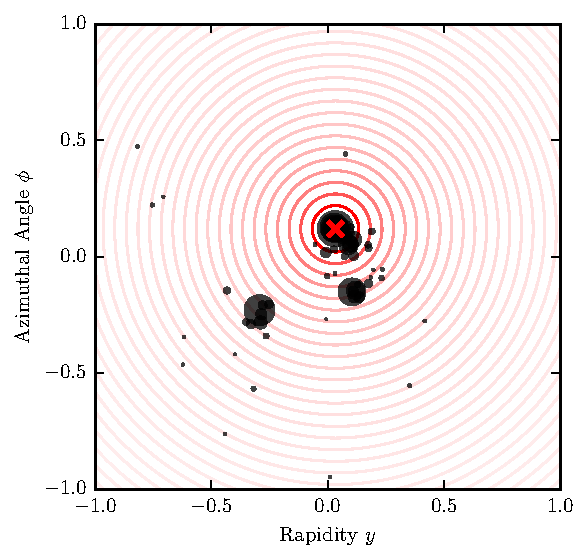
\includegraphics[width=.32\columnwidth]{figures/topjetT1_telescoped2.pdf}
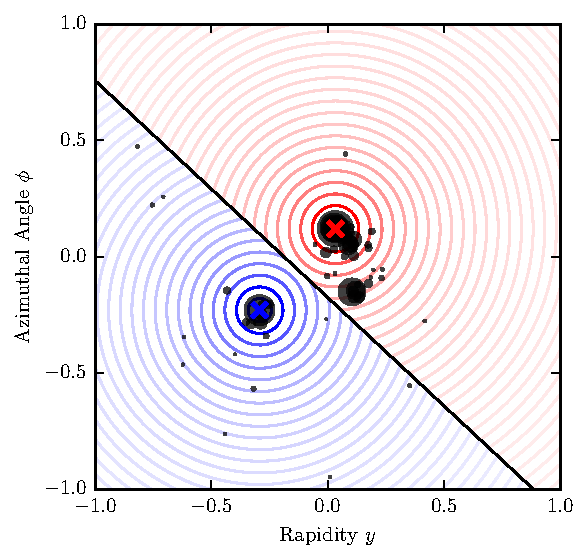
\includegraphics[width=.32\columnwidth]{figures/topjetT2_telescoped2.pdf}
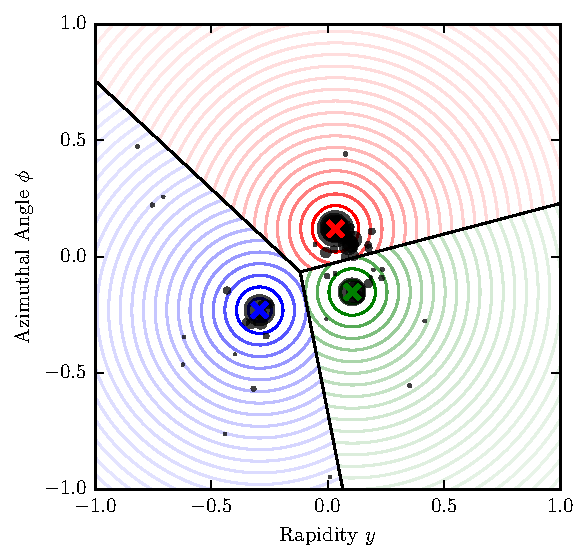
\includegraphics[width=.32\columnwidth]{figures/topjetT3_telescoped2.pdf}
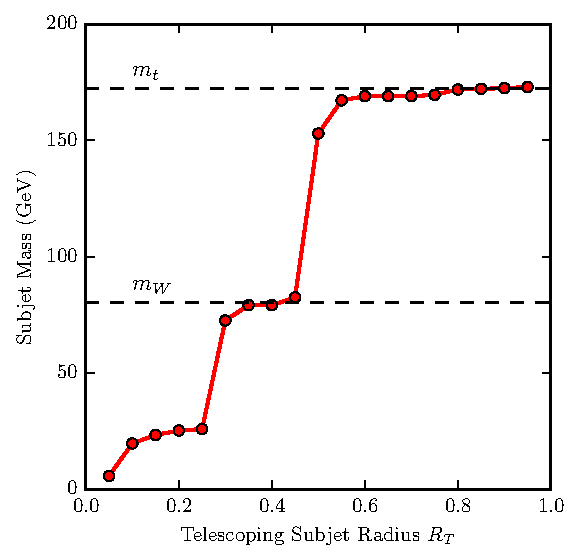
\includegraphics[width=.32\columnwidth]{figures/topjetT1_masses2.pdf}
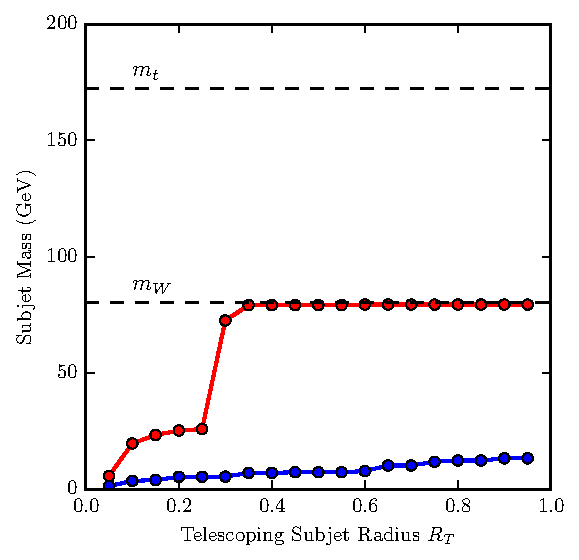
\includegraphics[width=.32\columnwidth]{figures/topjetT2_masses2.pdf}
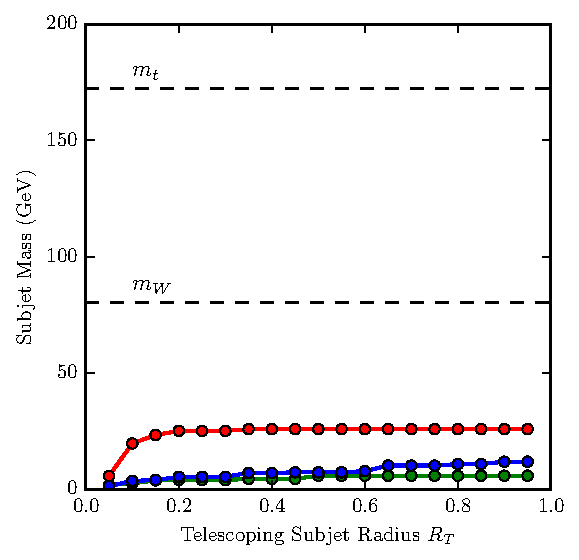
\includegraphics[width=.32\columnwidth]{figures/topjetT3_masses2.pdf}
\caption{\label{fig:tjet}(Top row) The telescoping deconstruction of a top jet at T1 (left panel), T2 (middle panel) and T3 (right panel) orders. The crosses are the Winner-Take-All $k_T$ axes. The straight lines are the exclusive subjet boundaries. Particles are sized according to their transverse momenta. (Bottom row) The subjet masses at T1 (left panel), T2 (middle panel), and T3 (right panel) orders as the telescoping radius $R_T$ is varied, corresponding to the region of the same color in the top row. The presence of the $W$ in the top jet can be clearly seen at T1 and T2 orders by the plateau of the red line beginning around $R_T=0.3$.}
\end{figure}

The telescoping deconstruction procedure is:
\begin{itemize}
        \item At order $N$, determine $N$ axes $\{\hat n_i\}=\{(\eta_i,\phi_i)\}$ along the dominant energy flows, where $y$ and $\phi_i$ are the rapidity and the azimuthal angle of the subjet axis $i$. We use the Winner-Take-All (WTA) $k_T$ axes \cite{Thaler:2010tr}.
        \item Construct $N$ subjets with $M$ radii $\{R_{T,m}\}^M_{m=1}$ by assigning particles to the nearest axis according to the distance $d^2_{ij} = \Delta y_{ij}^2+\Delta \phi_{ij}^2$ between the axis $\hat n_i$ and the particle $j$ \cite{Stewart:2010tn,Chien:2013kca,Stewart:2015waa,Thaler:2015xaa}.
            \begin{equation}
                {\rm subjet}_{i,m} = \{p^\mu_j~|~d_{ij}<R_{T,m}~{\rm and}~d_{ij}<d_{kj} \forall i\neq k\}.
            \end{equation}
            The subjet radii ${R_{T,m}}$ are sampled within the range $(0,R)$ where $R$ is the jet radius. In this paper $\{R_{T,m}\}$ are chosen to be evenly spaced within the range.
        \item We form the subjet data with the subjet transverse momenta and masses $\{(p_T,m)_{i,m}\}$,
            \begin{equation}
                {p_T}_{i,m}=\Big(\sum_{j\in~{\rm subjet}_{i,m}}p^\mu_j\Big)_T\;,~~~{m_{i,m}}^2=\Big(\sum_{j\in~{\rm subjet}_{i,m}}p^\mu_j\Big)^2\;,
            \end{equation}
            where we sum over all the particles $j$ within the subjet $i,m$. Together with the positions of the axes these form the telescoping deconstruction observables.
    \end{itemize}

The telescoping deconstruction observables fall into two categories~\cite{Chien:2017xrb}: the {\sl subjet topology}, which is described by the axes and subjet transverse momenta, and the {\sl subjet substructure}, quantified by the subjet masses. {\sl Subjet charge}~\cite{Krohn:2012fg} information can be included in this framework as well. As the telescoping subjet order $N$ (T$N$ order) increases, more jet energy is covered by the subjets and the number of subjet radii sampled can be systematically decreased. In the large $N$ limit, the subjets reduce to individual particles with the full jet information. The telescoping deconstruction allows one to exploit features both within each subjet and among all the subjets. See \Fig{fig:tjet} for the telescoping deconstruction of a top jet for $N = 1$, $2$, and $3$ where the $W$ resonance can clearly be seen.

To demonstrate the efficacy of telescoping deconstruction in capturing the full jet information,
we apply the framework in quark/gluon discrimination, boosted $W$ tagging and boosted top tagging. Each of these problems have
signal jets with a different characteristic number of prongs: one, two, and three prongs, respectively. Events were generated from Monte Carlo simulation of proton-proton collisions at 14 TeV using \textsc{Pythia} 8.226~\cite{Sjostrand:2007gs}. Final-state non-neutrino particles are clustered into jets with \textsc{FastJet} 3.3.0~\cite{Cacciari:2011ma} using the anti-$k_T$ algorithm~\cite{Cacciari:2008gp}. We consider the boosted regime with the jet $p_T$ between 800 GeV and 900 GeV. For quark/gluon discrimination, quark jets were generated by $pp\to q+Z(\to\nu\bar\nu)$ and gluon jets %were generated
by $pp\to g + Z(\to\nu\bar\nu)$, clustered into $R=0.4$ jets with rapidity $|y|<1.5$.

\begin{figure}[t]
\centering
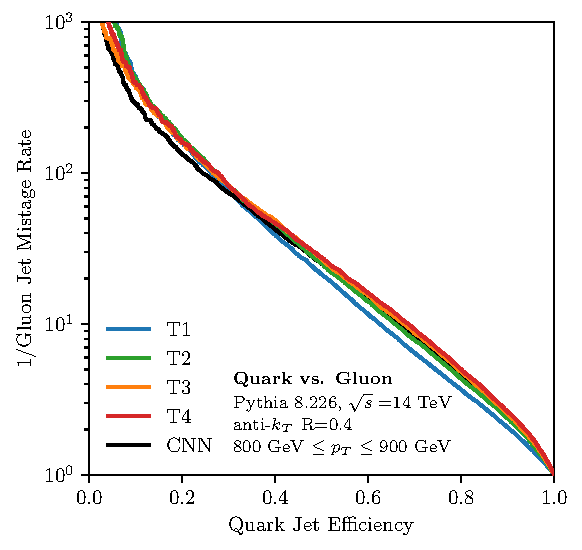
\includegraphics[width=.32\columnwidth]{figures/QG_invROC.pdf} 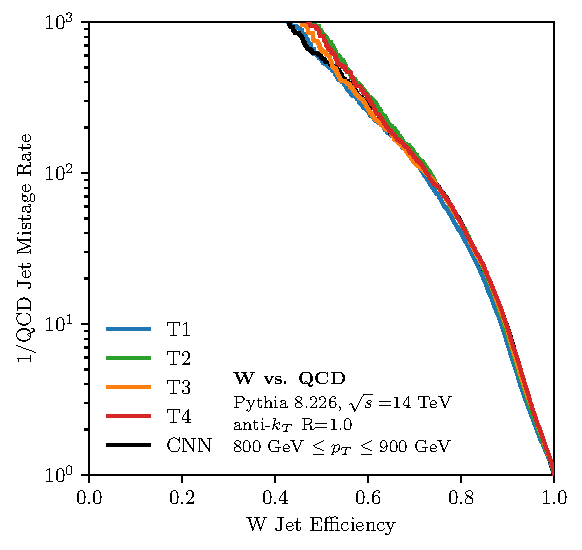
\includegraphics[width=.32\columnwidth]{figures/W_invROC.pdf} 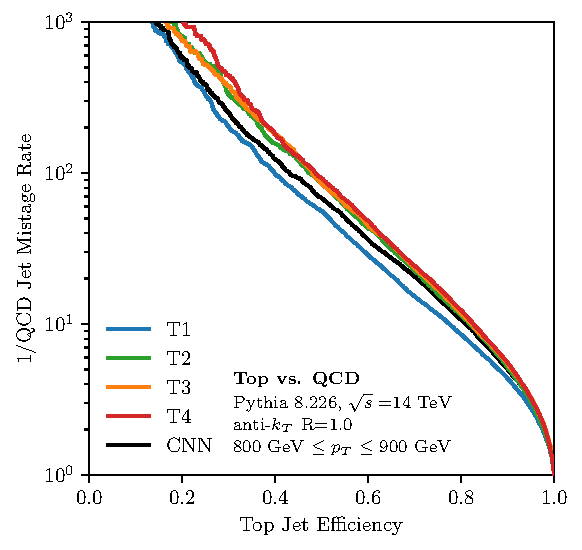
\includegraphics[width=.32\columnwidth]{figures/Top_invROC.pdf}
\caption{\label{ROCs}ROC curves for the DNNs trained on cumulant telescoping deconstruction observables up to T1 through T4 orders and the jet image method using CNNs for quark/gluon discrimination (left panel), boosted $W$ (middle panel) and top (right panel) tagging. The T$N$ performance approximately saturates at T2 (quark/gluon), T1 ($W$ tagging), and T2 (top tagging) orders.}
\end{figure}

Since $W$ and top tagging are mass resonance searches where the jet mass is the most natural and powerful discriminating variable, we disentangle mass information to probe how much additional information can be exploited for tagging. Information from the hard process about the overall jet kinematics is eliminated by translating each jet to a frame where $y$ and $\phi$ of the jet are both zero. For $W$ and top tagging, $W$ jets were generated by $pp\to WW (\to \text{hadrons})$ and top jets were generated by $pp\to t\bar t (\to \text{hadrons})$, with background jets from QCD dijets. Final-state non-neutrino particles are clustered into $R=1.0$ jets with rapidity $|y|<1.5$. Signal and background jets identically populate a five-bin $1/p_T^4$ histogram in transverse momentum and a three-bin uniform histogram in mass between 75 GeV and 85 GeV for $W$ tagging and 160 GeV to 180 GeV for top tagging. Telescoping subjets are constructed with $R_T$ in steps of 0.05 between 0.05 and 0.4 in
quark/gluon discrimination, and between 0.05 to 0.95 in
$W$ and top tagging. Reducing the number of radius sampling is left for future work. For each problem, 200k events are generated for signal and background, with 10\% used for validation, 15\% for testing, and the remaining 75\% for training.

A neural network consisting of three dense layers with 100 nodes each is trained on the telescoping deconstruction observables up to T$N$ order. The training can be performed on a typical laptop CPU in fewer than five minutes. One could also use boosted decision trees to combine variables \cite{Chien:2017xrb}. We compare the performance of our method to jet images using a CNN, which requires a graphics processing unit (GPU) to train. The jet images are size $33\times 33$ and span a $2R\times 2R$ patch of the rapidity-azimuth plane with the intensity of each pixel corresponding to the total $p_T$ of particles in the pixel. The jet images are standardized according to the procedure in \Ref{Komiske:2016rsd}. The CNN architecture consists of three 48-filter convolutional layers with filter sizes of $8\times 8$, $4\times 4$, and $4\times 4$ followed by a 128-unit dense layer and a 2-unit softmaxed output layer. A $2\times 2$ maxpooling is performed after each convolutional layer with a stride length of 2. The dropout rate was taken to be 0.1 for all layers. All neural networks are implemented using the Python deep learning library Keras~\cite{keras} with the Theano backend~\cite{bergstra2010theano}. Rectified linear unit (ReLU) activation functions~\cite{nair2010rectified} and He-uniform model weight initialization~\cite{heuniform} are used. The networks are trained using the Adam algorithm~\cite{adam} with a learning rate of $10^{-3}$ and a batch size of 256 for 50 epochs with a patience parameter of 8, and the best model is selected based on validation set performance.

The performance of the trained models can be captured in a Receiver Operating Characteristic (ROC) curve which plots the inverse of the background mistag rate at different signal efficiencies, where a higher curve indicates better classification performance. \Fig{ROCs} shows the ROC curves for the three tagging problems of the models trained on the cumulant telescoping deconstruction observables up to T$N$ order for $N\in\{1,2,3,4\}$ and the CNNs trained on jet images. The T$N$ performance converges quickly and is comparable to the performance of the jet images approach. % Note that since
The CNN architecture has not been tuned exhaustively, therefore its ROC curves serve to give a general sense of performance. %This is highlighted in the top case, where the telescoping deconstruction DNN outperforms the CNN at T2 order and above.
\begin{figure}
\centering
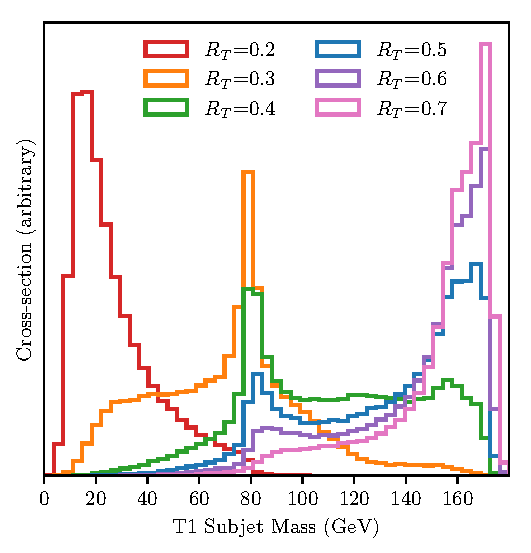
\includegraphics[width=.32\columnwidth]{figures/T1HeavyMass_top.pdf}
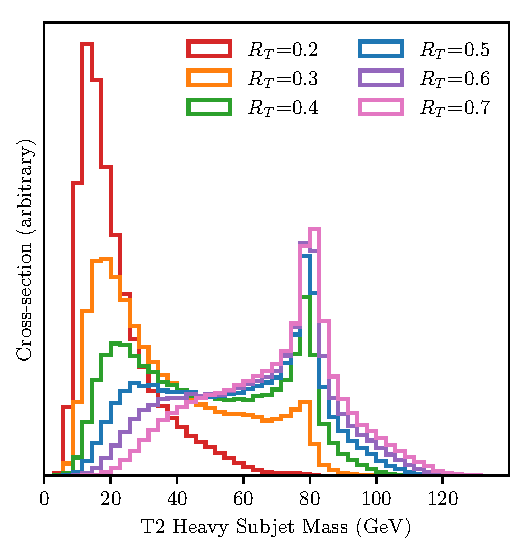
\includegraphics[width=.32\columnwidth]{figures/T2HeavyMass_top.pdf}
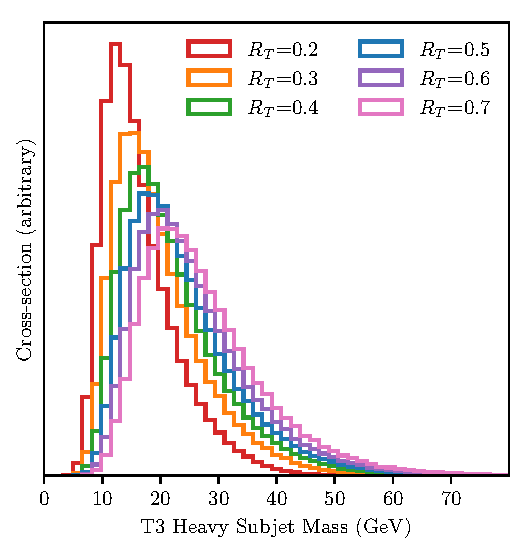
\includegraphics[width=.32\columnwidth]{figures/T3HeavyMass_top.pdf}
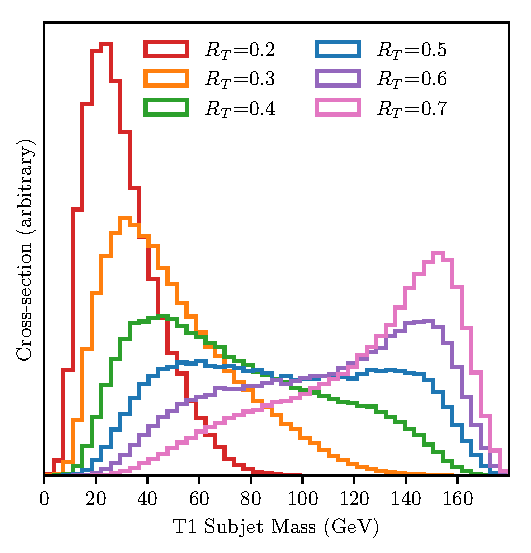
\includegraphics[width=.32\columnwidth]{figures/T1HeavyMass_qcd.pdf}
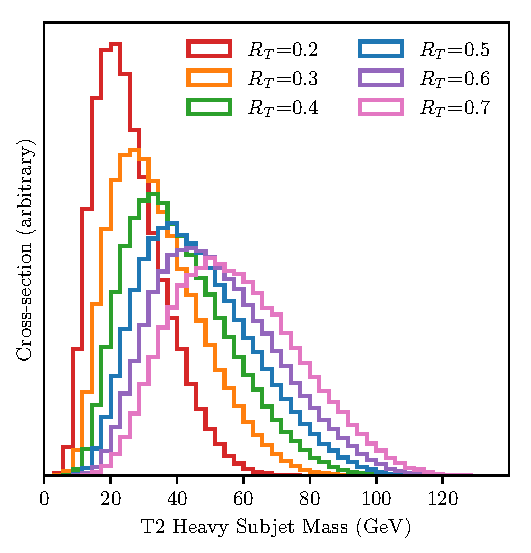
\includegraphics[width=.32\columnwidth]{figures/T2HeavyMass_qcd.pdf}
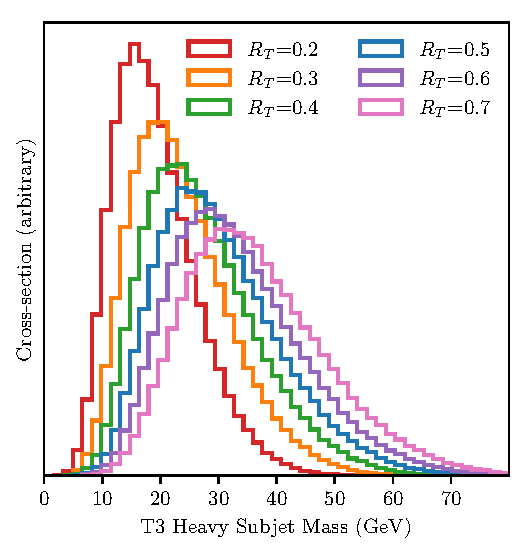
\includegraphics[width=.32\columnwidth]{figures/T3HeavyMass_qcd.pdf}
\caption{\label{masses}The heavy subjet mass distributions at T1 (left panels), T2 (middle panels), and T3 (right panels) orders for multiple subjet radii $R_T$ of top jets (top row) and QCD background jets (bottom row). The presence of the $W$ in top jets is evident by the peaks at the $W$ mass at T1 and T2 orders. At T3 order, the heavy subjet mass distributions are QCD-like and are narrower (more quark-like) in %the case of
top subjets than the wider (more gluon-like) QCD subjets. These features highlight the ability of the telescoping deconstruction to probe subjet substructure.}
\end{figure}

For top tagging, there is a significant increase in performance from T1 to T2 order in \Fig{ROCs}, and the performance saturates beyond this order due to the sensitivity of T2 to the $W$ in top jets. For $W$ tagging, T1 order is sufficient to achieve most of the classification performance, which unambiguously confirms the $W$ isolation feature in the boosted regime compared to the QCD background~\cite{Chien:2017xrb}. Clearly, the T1 order probes the depletion of the radiation at large angles within $W$ jets, whereas the QCD background jets continue to accrue mass from radiation at large angles. For quark/gluon discrimination, there is a significant increase in performance from T1 to T2 and a smaller increase from T2 to T3 where the performance saturates, suggesting the usefulness of T2 subjet substructure and its sensitivity to subjet flavors. This confirms that the T$N$ expansion converges efficiently and telescoping deconstruction faithfully represents the jet information.

In addition to being a useful jet representation, the telescoping deconstruction allows physical information to be easily extracted. \Fig{masses} shows the heavy subjet mass distributions at T1, T2, and T3 orders, scanned over different telescoping radii $R_T$, for top jets and their QCD background. As $R_T$ is increased, the top jet T1 subjet mass distributions transition from QCD-like, to peaked at the $W$ mass, to peaked at the top mass. In contrast, the background QCD jets do not peak at the $W$ mass for any $R_T$ and transition from QCD-like to more top-like as they %continue to
accrue mass at larger radii. The top jets at T2 order clearly and automatically show the $W$ peak which is completely absent in the background distributions. At T3 order, both top and background distributions appear QCD-like, with the wider background distributions %slightly wider
due to the prevalence of gluon subjets. This highlights again subjet substructure in telescoping deconstruction.

\bibliographystyle{JHEP3}
\bibliography{qg_ML_ref}

\end{document}

%We present the telescoping deconstruction framework as a complete, physically-motivated expansion of the jet. Neural networks were trained on the telescoping deconstruction observables up to different T$N$ orders and applied to quark/gluon discrimination, boosted $W$ and top tagging. Telescoping deconstruction observables up to different T$N$ orders are combined using multivariate methods and applied to quark/gluon discrimination, boosted $W$ and top tagging. The T$N$ performance converges efficiently and compares favorably to a CNN trained on jet images. Further, the individual telescoping deconstruction observables were shown to cleanly encode relevant features of jets such as the isolation of $W$ jets, the presence of the $W$ in top jets, and the quark- or gluon- like nature of the heaviest prongs in top and QCD jets. This complete and general framework is suitable for systematic studies of full jet dynamics, with rich future applications in parton-shower tuning, heavy ion hard probe studies, and identification of hadronic electroweak-boson emissions in ultra-high energy jets. The extension to hard-process tagging and resonance search at the event level is also promising.

    %layer = Convolution2D(8, 11, 11, border_mode='same')(input_layer)
    %layer = Activation('tanh')(layer)
    %layer = MaxPooling2D(pool_size=(2,2))(layer)
    %layer = Convolution2D(8, 3, 3, border_mode='same')(layer)
    %layer = Activation('tanh')(layer)
    %layer = MaxPooling2D(pool_size=(3,3))(layer)
    %layer = Convolution2D(8, 3, 3, border_mode='same')(layer)
    %layer = Activation('tanh')(layer)
    %layer = MaxPooling2D(pool_size=(3,3))(layer)
    %layer = Flatten()(layer)
    %layer = Dropout(0.20)(layer)
    %layer = Dense(20)(layer)
    %layer = Dropout(0.10)(layer)
    %output_layer = Dense(1, activation='sigmoid', name='main_output')(layer)
    %model = Model(input=input_layer, output=output_layer)
    %model.compile(optimizer='adam', loss='binary_crossentropy', metrics=['accuracy'])





























































